\documentclass[a4paper,UKenglish,cleveref,thm-restate]{lipics-v2021}
\nolinenumbers
\usepackage{float}

\title{Range Minimum Queries}

\author{Feyzi Eren Gündoğdu}{Karlsruhe Institute of Technology, Germany}{}{}{}
\authorrunning{F. Eren Gündoğdu}
\hideLIPIcs

\begin{document}
\maketitle


\section{Introduction}
This report compares the performance of 7 different data structures for Range Minimum Queries (RMQ) in C++.
The 7 data structures are: two naive baselines, \texttt{OnTheFlyNaive} and \texttt{PrecomputedNaive},
and five advanced structures, \texttt{SparseTable}, \texttt{SegmentTree}, \texttt{BlockSparseTable}, \texttt{BlockSparseTablePrecompute}
and \texttt{CartesianTree}.

Several of the advanced structures are parameterised by a block size $S$, and the different choices of $S$ are distinguished by a suffix in the implementation name.
For example, \texttt{AdBlPre200} denotes the Block Sparse Table with precomputed prefix and suffix minima and an adaptive block size $S = C \log_2 n$ with $C = 200$,
while \texttt{FiBl64} denotes the plain Block Sparse Table with a fixed block size of $64$.

All measurements were taken on inputs of size $n = 10^3$ to $3 \cdot 10^6$ with $2 \cdot 10^6$ queries each.
Construction time is excluded; only the time to answer all queries is measured and reported as the average time per query in nanoseconds.
The two naive baselines are only run up to $n = 10^4$, since
\texttt{PrecomputedNaive} would need roughly $20$\,GB of memory at $n = 10^5$ and
\texttt{OnTheFlyNaive} becomes prohibitively slow.

The submission contains the following files:
\begin{itemize}
	\item \texttt{main.cpp} contains all RMQ implementations.
	\item \texttt{benchmark.sh} is a shell script that runs the .cpp file 21 times and takes the median of the runs, writing the result to \texttt{data.csv}. Every measurement and figure in the report is from this implementation.
	\item \texttt{plot.py} produces the plots in \texttt{/plots} from \texttt{data.csv}.
	\item The \texttt{justfile} build and run everything.
	\item \texttt{report.tex} is the source of this report.
	\item \texttt{/plots} is the directory that stores all the figures.
\end{itemize}

\subsection{Experimental Setup}
All measurements reported here were produced on a single machine:

\begin{description}
	\item[Machine] Apple MacBook Pro M2 2022
	      \begin{itemize}
		      \item  Apple Silicon M2
		      \item ARM64/AArch64
		      \item  $4$ performance and $4$ efficiency cores
		      \item $8$\,GB of memory
	      \end{itemize}

	\item[Cache] Performace Cores
	      \begin{itemize}
		      \item  L1 instruction cache: 192 KiB per core
		      \item  L1 data cache: 128 KiB per core
		      \item   L2 cache: 16 MiB shared by the performance-core cluster
	      \end{itemize}

	\item[Cache]    Efficiency cores
	      \begin{itemize}
		      \item  L1 instruction cache: 128 KiB per core
		      \item  L1 data cache: 64 KiB per core
		      \item  L2 cache: 4 MiB shared by the efficiency-core cluster
	      \end{itemize}

	\item[Software] macOS Tahoe 26.2
	      \begin{itemize}
		      \item  Apple Clang 21.0.0
		      \item  \texttt{-std=c++17 -O3 -march=native -funroll-loops}.
	      \end{itemize}
\end{description}

\clearpage
\section{Methods}
\begin{table}[h]
	\centering
	\begin{tabular}{lcc}
		\hline
		Algorithm         & Space overhead (bits)                           & Query time                                                                           \\
		\hline
		OnTheFlyNaive     & $O(1)$                                          & $O(n)$                                                                               \\
		PrecomputedNaive  & $O(n^2 \log n)$                                 & $O(1)$                                                                               \\
		Sparse Table      & $O\!\left(n \log^2 n\right)$                    & $O(1)$                                                                               \\
		Segment Tree      & $O(n \log n)$                                   & $O(\log n)$                                                                          \\
		Blocks            & $O\!\left(\frac{n}{S}\log^2 n\right)$           & $O(S)$                                                                               \\
		Blocks Precompute & $O\!\left(n\log n + \frac{n}{s}\log^2 n\right)$ & $O(S)$$^{\ast}$ \\
			                                                                                    Cartesian Trees   & $O\!\left(\frac{n}{S}\log^2 n + 4^S S^2 \log S\right)$ & $O(1)$ \\
		\hline
	\end{tabular}
	\caption{Theoretical bounds. All space bounds exclude the input array and
		assume $\lceil \log_2 n \rceil$ bits per stored index; the implementations
		use a fixed width of $32$ bits per index instead, so every $\log n$ factor
		arising from index width is replaced by the constant $32$ in the measured
		values. $^{\ast}$For Blocks Precompute the query is $O(1)$ whenever the
		range spans a block boundary; the $O(S)$ bound applies only to ranges that
		lie inside a single block.}
	\label{tab:theoretical-bounds}
\end{table}

According to Table~\ref{tab:theoretical-bounds}, the smallest structure is \texttt{OnTheFlyNaive} with $O(1)$ overhead, at the cost of an $O(n)$ query.
Theoretically the fastest structures are \texttt{PrecomputedNaive},\texttt{Sparse Table},\texttt{Cartesian Trees} which all share $O(1)$ query time.
\subsection{OnTheFlyNaive}
\texttt{OnTheFlyNaive} (\texttt{NaiFly}) performs no preprocessing at all. The
structure consists of a single \texttt{const std::vector<uint64\_t>*} pointing at
the input array, so the reported space overhead is $\texttt{sizeof(*this)} = 8$
bytes, independent of $n$. A query $[l,r]$ is answered by a sequential
\texttt{std::min}. Unlike all other implementations, it returns the minimum value directly rather than its index.
This structure is only benchmarked up to $n = 10^4$.

\subsection{PrecomputedNaive}
\texttt{PrecomputedNaive} (\texttt{NaiPre}) stores the answer to every possible
query. For each pair $l \le r$ it stores the index of the minimum of the range
$[l,r]$, so only the upper triangular part of the full $n \times n$ table is
needed.
The table is kept as a single flat \texttt{std::vector<uint32\_t>} of length
$n(n+1)/2$ rather than as a nested vector of rows: the range $[l,r]$ is mapped to
the position
\[
	l \cdot n - \frac{l(l-1)}{2} + (r-l).
\]

A query is answered by one lookup into the table followed by one lookup into the
input array to fetch the value at the stored index, so the query time is $O(1)$.

Storing $\lceil \log_2 n \rceil$ bits per entry would give the bound
$O\!\left(\frac{n(n+1)}{2}\log n\right) = O(n^2 \log n)$ of
Table~\ref{tab:theoretical-bounds}. The implementation instead uses a fixed width
of $32$ bits per entry, so its actual space usage is
$32 \cdot \frac{n(n+1)}{2} = \Theta(n^2)$ bits; this is asymptotically smaller.
This structure is only benchmarked up to $n = 10^4$.

\subsection{SparseTable}
\texttt{SparseTable} (\texttt{SpTa}) stores a nested \texttt{std::vector<std::vector<uint32\_t>{}>} with $k+1$ levels, where $k = \lfloor \log_2 n \rfloor$.
Level $\ell$ holds one entry for every interval of length $2^\ell$ that fits into the input, that is $n+1-2^\ell$ entries, and each entry is the index of the minimum element of the corresponding interval.
Level $\ell$ is built from level $\ell-1$ by comparing two overlapping intervals of half the length, so construction takes $O(n \log n)$ time.
A query $[l,r]$ selects $\ell = \lfloor \log_2 (r-l+1) \rfloor$ and combines the two intervals of length $2^\ell$ starting at $l$ and ending at $r$, which together cover the range and may overlap.
The number of instructions per query is constant, so the query time is $O(1)$.

\subsection{SegmentTree}
\texttt{SegmentTree} (\texttt{SeTr}) stores, like the Sparse Table, indices of minima rather than the values themselves, but over disjoint intervals instead of all overlapping ones.
It is kept as a \texttt{std::vector<std::vector<uint32\_t>{}>} with one array per level:
level $0$ contains the $n$ input positions
and level $\ell$ contains $\lfloor n/2^\ell \rfloor$ entries,
each the index of the minimum of $2^\ell$ consecutive elements, built by pairwise comparison from level $\ell-1$.
The total number of stored entries is therefore below $2n$, so at $32$ bits per index the structure occupies at most $64n$ bits,
that is exactly $64$ bits per element independently of $n$.
This is the $O(n\log n)$ bits of Table~\ref{tab:theoretical-bounds} with the index width fixed to $32$,
and it is the reason the Segment Tree is substantially smaller in practice than the Sparse Table.

A query $[l,r]$ is answered bottom-up with two pointers.
At each level the algorithm checks whether the node containing $l$ is a right child and whether the node ending at $r$ is a left child;
in each case the corresponding node lies entirely inside the query range, its index is merged into the running candidate, and the pointer is moved inward by one block.
The block size is then doubled and the next level is considered, so at most two nodes per level are inspected and the query time is $O(\log n)$.

\subsection{BlockSparseTable}
\texttt{BlockSparseTable} (\texttt{Bl}) partitions the input into blocks of $S$ consecutive elements.
Level $0$ of the structure stores, for each of the $\lceil n/S\rceil$ blocks, the index of its minimum.
Over this array of block minima a single sparse table is built:
level $k$ stores the position of the minimum over $2^k$ consecutive blocks,
computed as $T[k][j]=\arg\min\big(T[k-1][j],\,T[k-1][j+2^{k-1}]\big)$.
The table therefore occupies $O\!\left(\frac{n}{S}\log\frac{n}{S}\right)$ words;
for $S=\Theta(\log n)$ this is $O(n)$.
The whole structure is a \texttt{std::vector<std::vector<uint32\_t>{}>} holding global indices into the input array.

A query $[l,r]$ is answered in three parts.
Let $b_l=\lfloor l/S\rfloor$ and $b_r=\lfloor r/S\rfloor$.
If $b_l=b_r$ the range lies inside one block and is scanned directly.
Otherwise the suffix of block $b_l$ and the prefix of block $b_r$ are scanned element by element, costing at most $S-1$ comparisons each,
while the blocks strictly between them are covered by two overlapping sparse-table lookups at level $k=\lfloor\log_2(b_r-b_l-1)\rfloor$.
The spanning part is thus $O(1)$ and the query is $O(S)$ overall.

For $S=\Theta(\log n)$ the bounds match those of the segment tree, but the
constant factors differ: the spanning part costs two table lookups.
Two ways of choosing $S$ are evaluated:

\begin{itemize}
	\item \emph{FiBl}: fixed $S$, given as a template parameter. Powers of two are used.
	\item \emph{AdBl}: $S=\ C\log_2 n$ for several constants $C$.
\end{itemize}

\subsection{BlockSparseTablePrecompute}
\texttt{BlockSparseTablePrecompute} (\texttt{BlPre}) uses the same block decomposition and the same sparse table over block minima as \texttt{BlockSparseTable},
and adds two arrays \texttt{prefixMin} and \texttt{suffixMin}, each a \texttt{std::vector<uint32\_t>} of length $n$.
For very position $i$, \texttt{prefixMin}$[i]$ is the index of the minimum of the range from the start of $i$'s block up to $i$,
and \texttt{suffixMin}$[i]$ the index of the minimum from $i$ to the end of its block.
Both are computed in a single linear pass per block during construction.
The query changes only in its partial-block part.
For $b_l \neq b_r$, the suffix of block $b_l$ and the prefix of block $b_r$ are no longer scanned but read directly as $\min\big(p[\texttt{suffixMin}[l]],\, p[\texttt{prefixMin}[r]]\big)$,
so the query becomes $O(1)$.
The $O(S)$ bound survives only for ranges with $b_l = b_r$, which still have to be scanned element by element.
The two arrays hold $2n$ indices and therefore dominate the space usage: at $32$
bits per index the structure needs $64$ bits per element plus the
$O\!\left(\frac{n}{S}\log\frac{n}{S}\right)$ words of the sparse table, which is
negligible for the block sizes considered here.

In this variant three ways of selecting $S$ is implemented:

\begin{itemize}
	\item \emph{FiBlPre}: fixed $S$, given as a template parameter. Powers of two are used.
	\item \emph{AdBlPre}: $S=\ C\log_2 n$ for several constants $C$.
	\item \emph{SqrtBlPre}: $S=\ C\ \sqrt{n}$ for several constants $C$.
\end{itemize}


\subsection{CartesianTree}
\texttt{CartesianTree} (\texttt{Cart}) uses the same block decomposition and the same sparse table over block minima as the previous two structures,
but replaces the scanning of partial blocks by table lookups.
The key observation is that the answer to an in-block query depends only on the \emph{shape} of the Cartesian tree of that block, not on the values themselves, and that the number of distinct
shapes of a block of size $S$ is the Catalan number $C_S = O(4^S)$.
Rather than building the trees, each block is encoded by a $2S$-bit representations(\texttt{code}).
For each distinct code, one row of a lookup table is stored, containing the block-local index of the minimum for all $S(S+1)/2$ pairs $(a,b)$ with $a \le b$,
in the same triangular layout used by \texttt{PrecomputedNaive}.
Rows are materialised lazily: a \texttt{std::unordered\_map<uint64\_t, uint32\_t>} maps
each code to the index of its row, and a row is built only when its shape is
encountered for the first time. The number of rows is therefore bounded by
$\min\!\left(C_S, \lceil n/S\rceil\right)$ rather than by $C_S$, which keeps the lookup
table small even when $4^S$ is large compared to $n$.

A query $[l,r]$ with $b_l = b_r$ is answered by a single lookup into the row of block $b_l$.
Otherwise the suffix of block $b_l$ and the prefix of block $b_r$ are obtained by one lookup each, and the blocks in between by the usual two
sparse-table lookups. Every query is therefore $O(1)$, including the in-block case,
which distinguishes this structure from both block variants.

We have 2 ways of selecting $S$:
\begin{itemize}
	\item \emph{FiCart}: fixed $S$, given as a template parameter. Powers of two are used.
	\item \emph{AdCart}: $S=\ C\log_2 n$ for several constants $C$.
\end{itemize}

\section{Results}

\subsection{OnTheFlyNaive}
\subsubsection{Space}
In the bits-per-element plot in \hyperref[fig:space]{Figure~\ref*{fig:space}}, the space usage appears to converge to $0$.
This is expected, because the method uses only constant additional space.
In this implementation, the only stored data is a pointer to the input array, which takes exactly $8$ bytes.
Therefore, the plotted value is $64/n$ bits per element, which tends to $0$ as $n$ grows.
So, the space usage remains constant at $64$ bits, matching the theoretical $O(1)$ extra space bound.
\subsubsection{Time}
The query time in \hyperref[fig:time]{Figure~\ref*{fig:time}} grows with $n$, which is consistent with the $O(n)$ worst-case query time.
This is because each query is answered by scanning the queried range directly.


\subsection{PrecomputedNaive}
\subsubsection{Space}
The results from \texttt{data.csv} indicate that the measured space usage matches
the expected implementation-level bound. For example, for $n = 10000$, the table
contains
\[ \frac{10000 \cdot 10001}{2} \]
entries. Since each entry is stored as a \texttt{uint32\_t}, each entry occupies
$4$ bytes. Therefore, the expected space usage is approximately
\[
	4 \cdot \frac{10000 \cdot 10001}{2}
	=
	200020000
\]
bytes, plus a small constant overhead. This matches the measured value
$200020040$ bytes.
Although the curve appears almost linear in the log-log \hyperref[fig:space]{Figure~\ref*{fig:space}}, this does not indicate linear space growth in $n$.
The measured space usage of PrecomputedNaive is proportional to
\[
	32 \cdot \frac{n(n+1)}{2}
\]
bits, which is $\Theta(n^2)$. On a log-log plot, polynomial growth appears as a
straight line; in this case, the slope corresponds to quadratic growth.

\subsubsection{Time}
For the query time, the theoretical $O(1)$ bound is only approximately visible
in the measurements. Each query performs a constant number of lookups, one into
the table and one dependent lookup into the input array, but
the measured running time is affected by cache and memory hierarchy effects as
the table grows. Nevertheless, \hyperref[fig:time]{Figure~\ref*{fig:time}}
shows that \texttt{PrecomputedNaive} behaves near-constantly.
The query time increases sharply from $n=1000$ to $n=3000$,
but grows more slowly afterwards. This is explained by the cache hierarchy: the
table occupies $2.0$\,MB at $n=1000$ and still fits into the $16$\,MiB L2 cache,
whereas at $n=3000$ it occupies $18.0$\,MB and no longer does, which is exactly
where the query time jumps from $0.87$\,ns to $3.72$\,ns.
Once the table exceeds the relevant cache levels, random table lookups
become much more expensive. After this point, the queries are already mostly
memory-latency bound, so increasing $n$ further does not lead to a
proportional increase in query time; at $n=10^4$ the table is $200$\,MB and the
query time only rises to $5.89$\,ns. Thus, the observed behavior is consistent
with an $O(1)$ query algorithm affected by the memory hierarchy.


\subsection{SparseTable}
\subsubsection{Space}
Numerically, the measurements from \texttt{data.csv} follow the theoretical bounds discussed above:
the closed form predicts $287.58$ bits per element at $n=10^3$ and $659.26$ at $n=3\cdot10^6$, against measured values of $287.84$ and $659.26$.
The behavior in \hyperref[fig:space]{Figure~\ref*{fig:space}} is also consistent with the theory.
Since this plot shows the space usage normalized by the input size, the expected growth for the sparse table is
\[
	\frac{O(n \log n)}{n} = O(\log n).
\]
Thus, the slow increase in bits per element matches the expected logarithmic growth.
\subsubsection{Time}
For the query time analysis, \hyperref[fig:time]{Figure~\ref*{fig:time}} shows that the sparse table has almost constant query time for the smaller input sizes, which is consistent with the theoretical $O(1)$ query bound.
For larger input sizes, however, the measured query time increases.
This does not contradict the theoretical complexity.
A sparse table query still performs the same constant number of memory accesses: two into the table, and two dependent ones into the input array to compare the corresponding values.
The increase in running time is caused by practical hardware effects.
As the input size grows, the sparse table becomes too large to fit into the CPU caches: it occupies $6.3$\,MB at $n=10^5$ and still fits into the $16$\,MiB L2 cache, but $20.7$\,MB at $n=3\cdot10^5$, which is where the measured time rises from $2.17$\,ns to $3.51$\,ns.
Consequently, all four accesses are more likely to cause cache misses and main-memory accesses, which have higher latency.
Thus, the measured running time increases due to memory hierarchy effects.

\subsection{SegmentTree}
\subsubsection{Space}
Numerically, the algorithm behaves in line with the theoretical space bound.
It displays the expected linear behavior with a small constant factor, as can be seen in \hyperref[fig:space]{Figure~\ref*{fig:space}}.
The total number of stored indices is bounded by $2n$ for an input of size $n$.
Since each stored index is a \texttt{uint32\_t} and requires $4$ bytes, the space usage is bounded by $8n$ bytes, that is exactly $64$ bits per element; the measured value is $64.00$ bits per element for every $n$.
\subsubsection{Time}
For the query time analysis, \hyperref[fig:time]{Figure~\ref*{fig:time}} shows that the algorithm is noticeably slower than Sparse Table.
This is expected because Sparse Table answers queries with a constant number of table accesses.
In contrast, this Segment Tree implementation performs repeated branching and level-by-level traversal during each query.
The measurements do follow the theoretical $O(\log n)$ bound: a linear fit over $n=10^3$ to $10^6$ gives about $12.3$\,ns per level with a deviation below $5\%$.
Only the last point at $n=3\cdot10^6$ breaks out of this trend, at $293$\,ns instead of the predicted $208$\,ns, since the input array alone occupies $24$\,MB there and no longer fits into the $16$\,MiB L2 cache.

\subsection{BlockSparseTable}
\subsubsection{Block Size Selection}
For choosing $S$, two families were compared. The results showed that fixed block size of 64 was the best choice. See Appendix~\ref{app:block-selection-nonprecompute} for detailed figures.
\texttt{FiBl} where fixed sized powers of 2 were tried and \texttt{AdBl} where different values of a constant were tested for $C \log n$.
The optimum is a compromise between the two parts of the query: a smaller $S$ shortens the two partial-block scans but enlarges the sparse table above them, which is accessed randomly, while a larger $S$ shrinks the table at the cost of longer scans.
There is a caveat here; because of the implementation the fixed block sizes are known at compile time, so the divisions by $S$ in the query become shifts, whereas the adaptive block size is only known at runtime and costs two integer divisions per query.
The effect of such a discrepancy between the families because of this didn't change the outcome.
The fixed sized family dominated the adaptive size familiy over all sample sizes up to $3 \cdot 10^6$.
From the progression of the families over increasing $n$ it can be seen that adaptive size family would be Pareto Optimal at higher values for $n$ but for our current range of $n$ fixed sized 64 is the final decision for block size.

\subsubsection{Space}
The space per element grows slowly with $n$, as can be seen in \hyperref[fig:space]{Figure~\ref*{fig:space}}.
As discussed previously the structure stores one index per block at level $0$, that is $\lceil n/S \rceil$ entries, and a sparse table of $\log \frac{n}{S}$ further levels above it.
Since $S$ is fixed, this is $\Theta(n \log n)$ bits in total, so the space per element grows logarithmically rather than staying constant
\subsubsection{Time}
For the query time analysis, \hyperref[fig:time]{Figure~\ref*{fig:time}} shows that the query time is essentially constant, between $24.20$ and $24.53$\,ns for all $n$ up to $10^6$, as expected for a fixed $S$ with an $O(S)$ query.
The only exception is the last point at $n=3 \cdot 10^6$, where it rises to $40.30$\,ns; there the input array alone occupies $24$\,MB and no longer fits into the $16$\,MiB L2 cache, so the block scans start to miss.

\subsection{BlockSparseTablePrecompute}
\subsubsection{Block Size Selection}
For choosing $S$, three families were compared in an intra- and inter-family fashion.
In Appendix~\ref{app:block-selection-precompute} there is an overall comparison for the winners and their neighbors from each family.
In Appendix~\ref{app:block-selection-precompute-fixed}, Appendix~\ref{app:block-selection-precompute-adaptive} and Appendix~\ref{app:block-selection-precompute-sqrt} the intra-family comparison of the families can be seen.
From these figures the selection for the block size is adaptive block size selection with $C$ being $200$.
Note that within this family the choice of $S$ is a one-dimensional decision: the prefix and suffix arrays dominate the space usage and their size does not depend on $S$, so all variants occupy essentially the same $64$ bits per element and differ only in query time.
The optimum lies at a much larger $S$ than for \texttt{BlockSparseTable}, since a cross-block query no longer scans the partial blocks at all, so a large $S$ costs nothing except for the queries that fall inside a single block.
\subsubsection{Space}
The algorithm displays linear space usage in \hyperref[fig:space]{Figure~\ref*{fig:space}}, and it requires more space than the non-precompute variant since it also stores the prefix and suffix minima.
These two arrays hold $2n$ indices of $32$ bits each and therefore fix the space usage at $64$ bits per element, independently of $n$ and of $S$; the sparse table above them contributes only $0.06$ bits per element at $n = 3 \cdot 10^6$.
The measured values confirm this, falling from $64.93$ bits per element at $n=10^3$ to $64.06$ from $n=10^5$ on, where the constant overhead of the structure itself becomes negligible.
\subsubsection{Time}
For the query time analysis, \hyperref[fig:time]{Figure~\ref*{fig:time}} shows a rise up to $n=3 \cdot 10^3$ followed by a long decrease, with a minimum of $4.66$\,ns at $n=3 \cdot 10^5$.
The reason is that $S = 200 \log_2 n$ is very large for small $n$: at $n=10^3$ the block size is $1993$, so the entire input forms a single block and every query degenerates to a linear scan.
This is confirmed by the measurement, $47.24$\,ns against $47.40$\,ns for \texttt{OnTheFlyNaive} on the same input.
At $n=3 \cdot 10^3$ there are two blocks and the time is roughly half that of the naive scan, $71.05$\,ns against $150.59$\,ns.
As $n$ grows further the fraction $S/n$ of queries that fall inside one block shrinks and more queries take the $O(1)$ path, so the time drops until the prefix and suffix arrays, $24$\,MB at $n=3 \cdot 10^6$, exceed the $16$\,MiB L2 cache and it rises again to $10.64$\,ns.


\subsection{Cartesian}
\subsubsection{Block Size Selection}
For choosing $S$, two families were compared.
The behaviour of the families was clear enough that an inter-family comparison was unnecessary.
There is one value in each family that outperforms the rest.
In Appendix~\ref{app:block-selection-cartesian} a clear selection for the block-size value from each family can be seen as fixed size of $8$ and adaptive constant $0.5$.
Since one value is needed for the comparison, fixed size of $8$ is selected.
Both winners describe almost the same block size over the measured range, since $0.5 \log_2 n$ lies between $5$ and $11$ for $n$ between $10^3$ and $3 \cdot 10^6$, which is why the two families behave so similarly.

\subsubsection{Space}
The space per element is nearly flat for small $n$ and grows slowly for large $n$, as can be seen in \hyperref[fig:space]{Figure~\ref*{fig:space}}.
The structure consists of three parts, of which the sparse table over the $\lceil n/S \rceil$ block minima dominates: at $n = 3 \cdot 10^6$ it accounts for $26.4$\,MB, against $1.5$\,MB for the shape indices and only $51$\,KB for the lookup table, giving the measured $27954944$ bytes in total.
At small $n$ the curve is not yet monotone, since the constant cost of the lookup table is amortised over few elements and initially outweighs the logarithmic growth.

\subsubsection{Time}
The query time is nearly constant at $2.4$ to $4.5$\,ns for $n$ up to $3 \cdot 10^5$, which matches the theoretical $O(1)$ bound and makes this the only structure that answers in-block queries without any scan.
It is nevertheless slower than the Sparse Table over the same range, because a cross-block query performs three lookups into the lookup table and the sparse table on the first level and up to four dependent accesses into the input array on the second, against two and two for the Sparse Table.
The slow rise up to $3 \cdot 10^5$ follows the growth of the structure rather than the instruction count, and at $n = 3 \cdot 10^6$ the query time jumps to $17.71$\,ns, where the structure at $28$\,MB and the input array at $24$\,MB both exceed the $16$\,MiB L2 cache.
At that size it is outperformed by \texttt{AdBlPre200}, which needs $10.64$\,ns at a comparable $64$ bits per element, so the asymptotic advantage predicted by the theory does not materialise within the measured range.

\subsection{Overall}
From \hyperref[fig:tradeoff81]{Figure~\ref*{fig:tradeoff81}} and \hyperref[fig:tradeoff82]{Figure~\ref*{fig:tradeoff82}}:

\texttt{PrecomputedNaive} is the fastest only at $n = 1000$, where its table still fits into the cache.

\texttt{SparseTable} is the fastest between $n = 3000$ and $n = 3{,}000{,}000$, with the only outlier being $n = 1{,}000{,}000$, where \texttt{AdBlPre200.00} is faster at $4.95$\,ns against $7.26$\,ns; \texttt{FiCart8} also overtakes it there.

For Pareto optimality only \texttt{FiBl64} stays on the Pareto front across all values of $n$.
\texttt{SparseTable} is on the front at every size except $n = 10^6$, and \texttt{FiCart8} up to $n = 3 \cdot 10^5$, after which \texttt{AdBlPre200.00} dominates it in both space and time.
\texttt{SegmentTree} is on the front at no size at all: \texttt{AdBlPre200.00} occupies the same $64$ bits per element and is faster at every $n$, by a factor of $28$ at $n = 3 \cdot 10^6$.

The best choice therefore depends on the objective.
For small space, \texttt{FiBl64} is the clear winner at $7.30$ bits per element and $40.30$\,ns at $n = 3 \cdot 10^6$, an order of magnitude smaller than anything else with a comparable query time.
For speed, \texttt{SparseTable} is the best choice, but at $n = 3 \cdot 10^6$ it buys only $0.5$\,ns over \texttt{AdBlPre200.00} for ten times the space.
As a general-purpose balanced trade-off \texttt{AdBlPre200.00} is selected: it is on the Pareto front at the two largest sizes, needs a constant $64$ bits per element independently of $n$, and stays within a factor of two of the fastest method over the whole measured range.

Notably, the structure that the theory favours is not the one that wins.
\texttt{CartesianTree} is the only method combining $O(1)$ queries with $O(n \log n)$ bits, yet at $n = 3 \cdot 10^6$ it is slower than \texttt{AdBlPre200.00} at comparable space, because its queries perform more dependent random accesses and its space is dominated by the same sparse table the other block structures use.

\subsection{Hardware Effects}
For the purposes of this report the cache sizes of the hardware are the dominant bottleneck.
Every method in \hyperref[fig:time]{Figure~\ref*{fig:time}} is flat or near-flat while its data structure fits into the $16$\,MiB L2 cache and bends upwards at the size where it no longer does, and for the larger structures this happens within the measured range: \texttt{NaiPre} between $n = 10^3$ and $3 \cdot 10^3$, \texttt{SpTa} between $10^5$ and $3 \cdot 10^5$, and \texttt{FiBl64}, \texttt{AdBlPre200.00}, \texttt{FiCart8} and \texttt{SeTr} at $n = 3 \cdot 10^6$, where the input array alone occupies $24$\,MB.
Asymptotic complexity is therefore a poor predictor of the measured ranking, since all the $O(1)$ methods perform the same constant number of instructions at every $n$ and differ only in how many of their accesses miss.


Further optimisations can be done by using bitpacking for storing the indices and possibly utilizing parrellization on the memory accsesses using $SIMD$ like instructions,but the Apple M2 implements NEON without a gather instruction, so it is not available here.

\begin{figure}[ht]
	\centering
	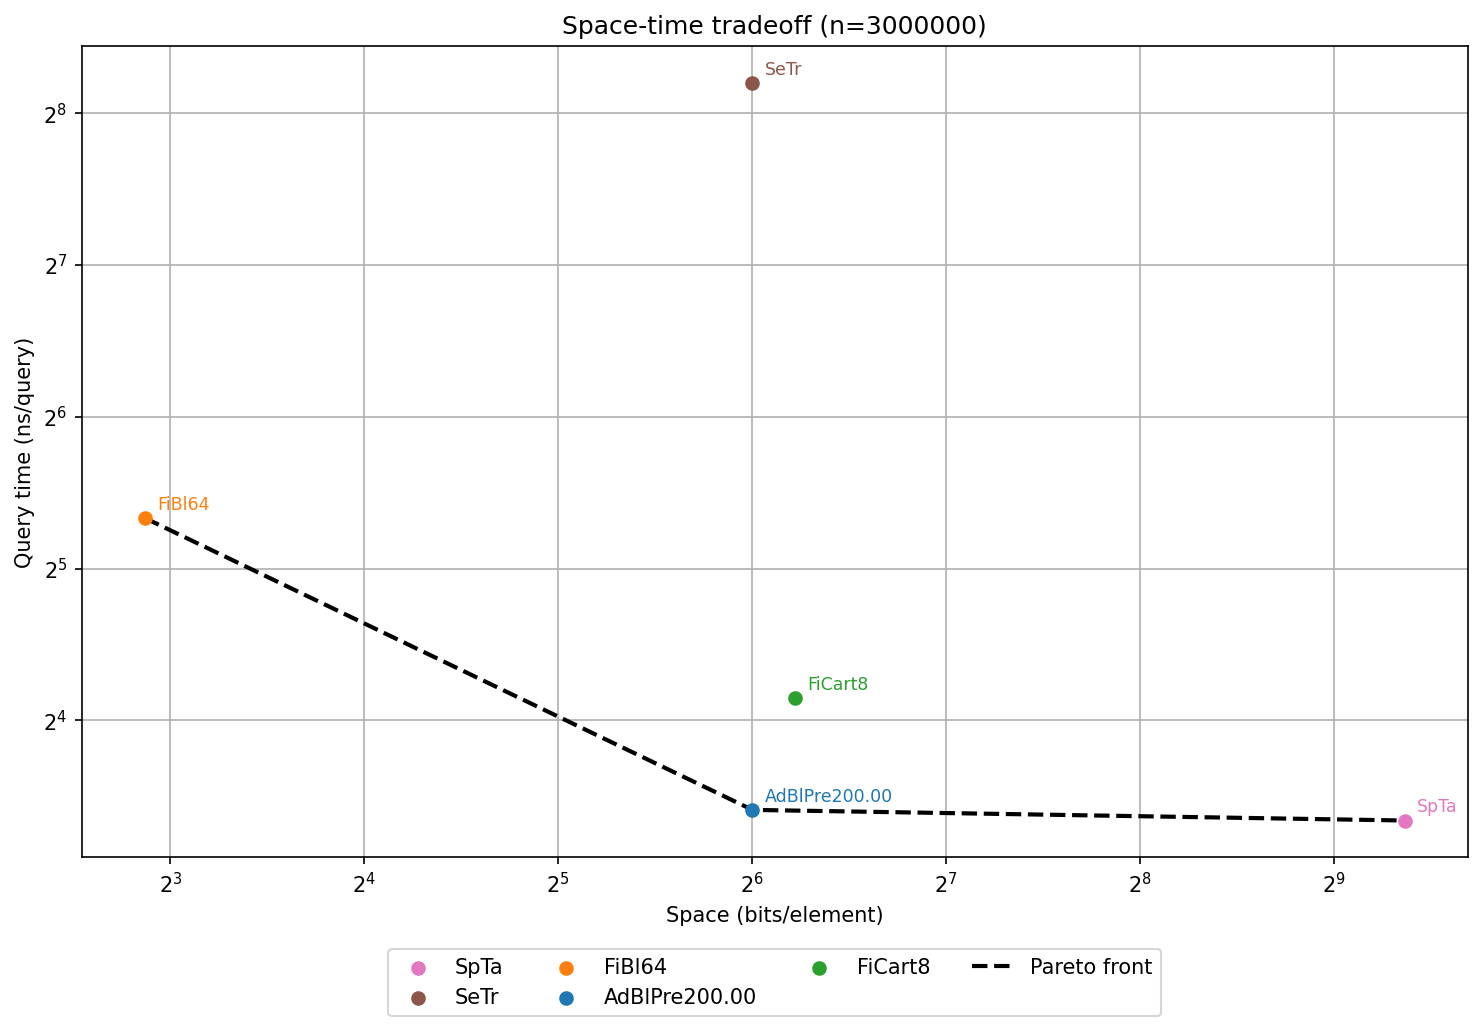
\includegraphics[width=.8\linewidth]{../plots/main/space_time_tradeoff.png}
	\caption{space-time trade-off}
	\label{fig:tradeoff}
\end{figure}
\begin{figure}[ht]
	\centering
	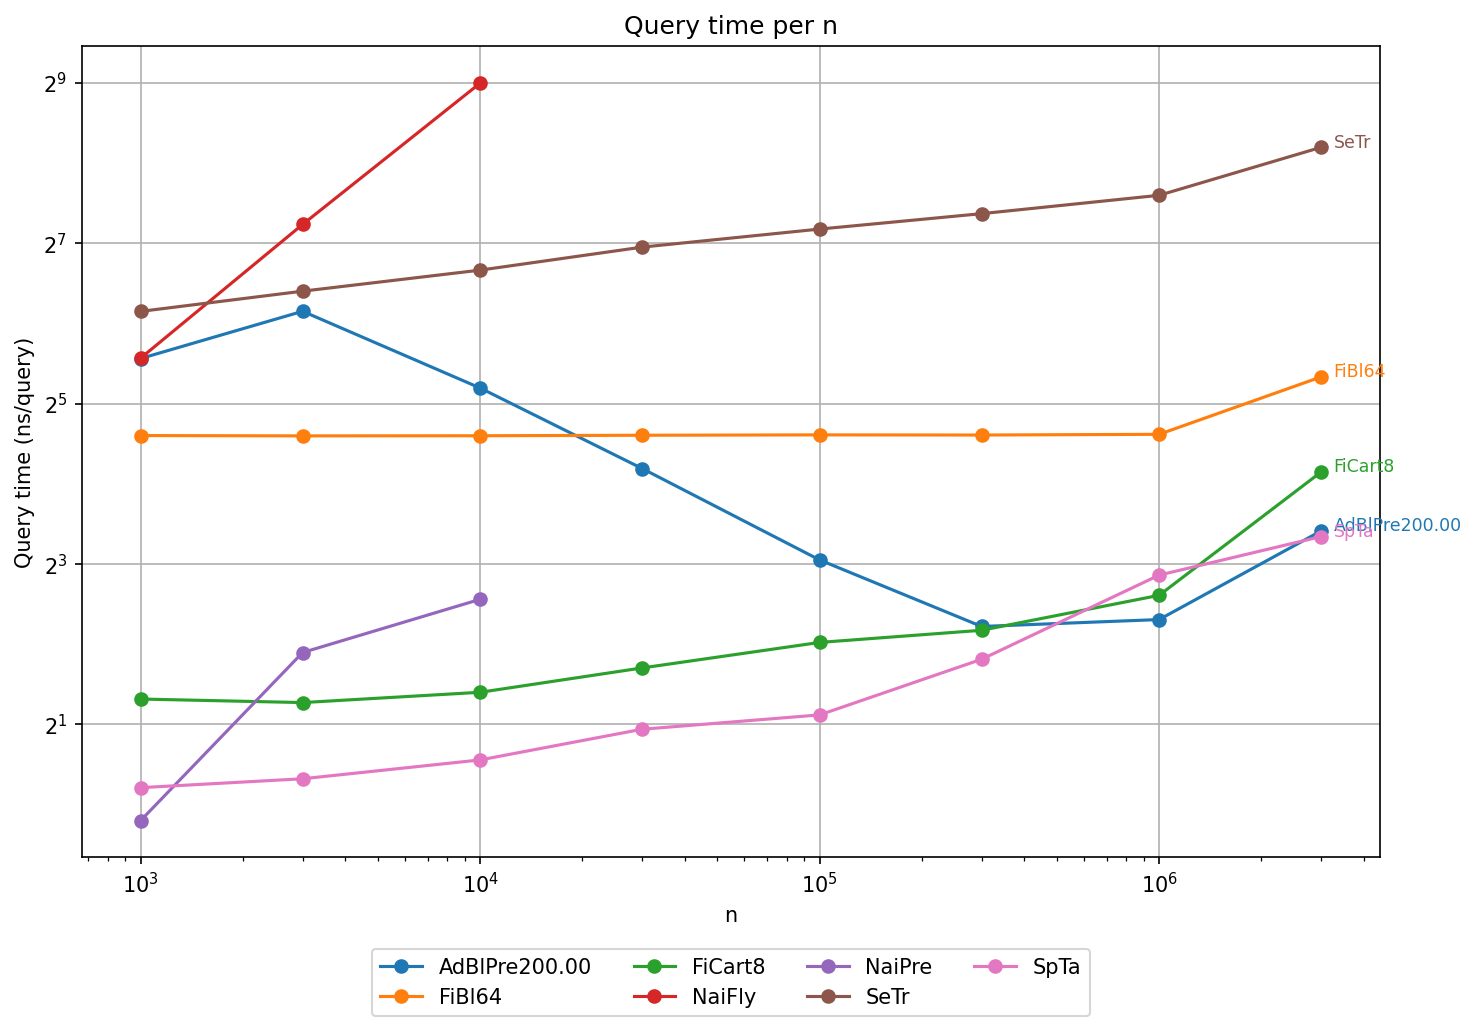
\includegraphics[width=.8\linewidth]{../plots/main/query_time.png}
	\caption{query time}
	\label{fig:time}
	\centering
	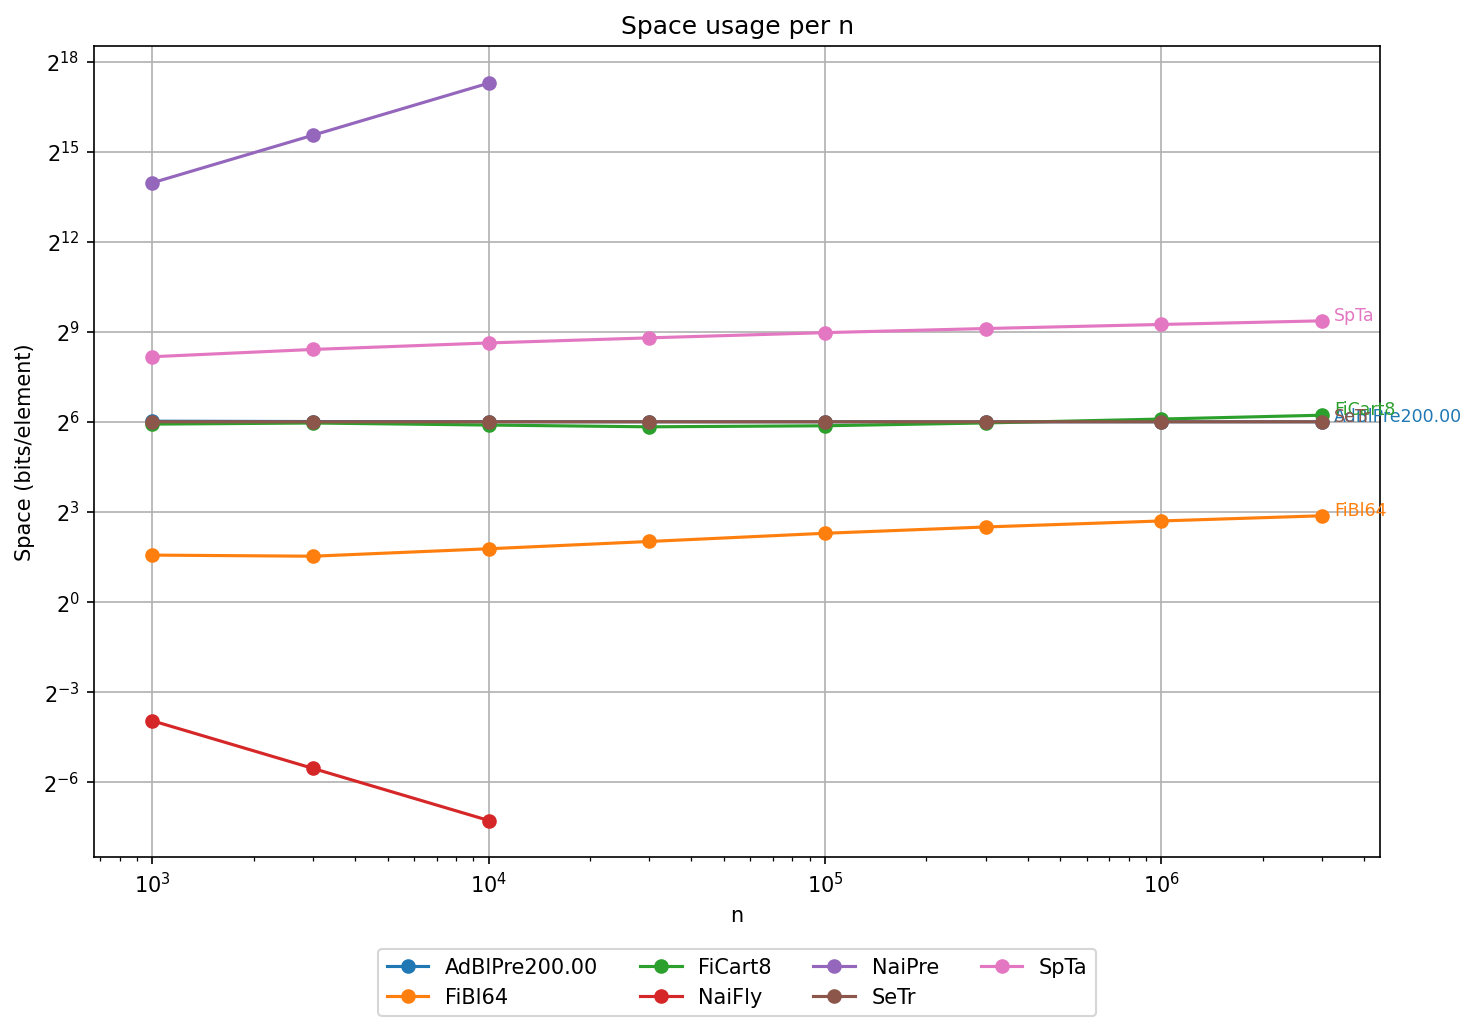
\includegraphics[width=.8\linewidth]{../plots/main/space.png}
	\caption{space usage}
	\label{fig:space}
\end{figure}
\begin{figure}[ht]
	\centering
	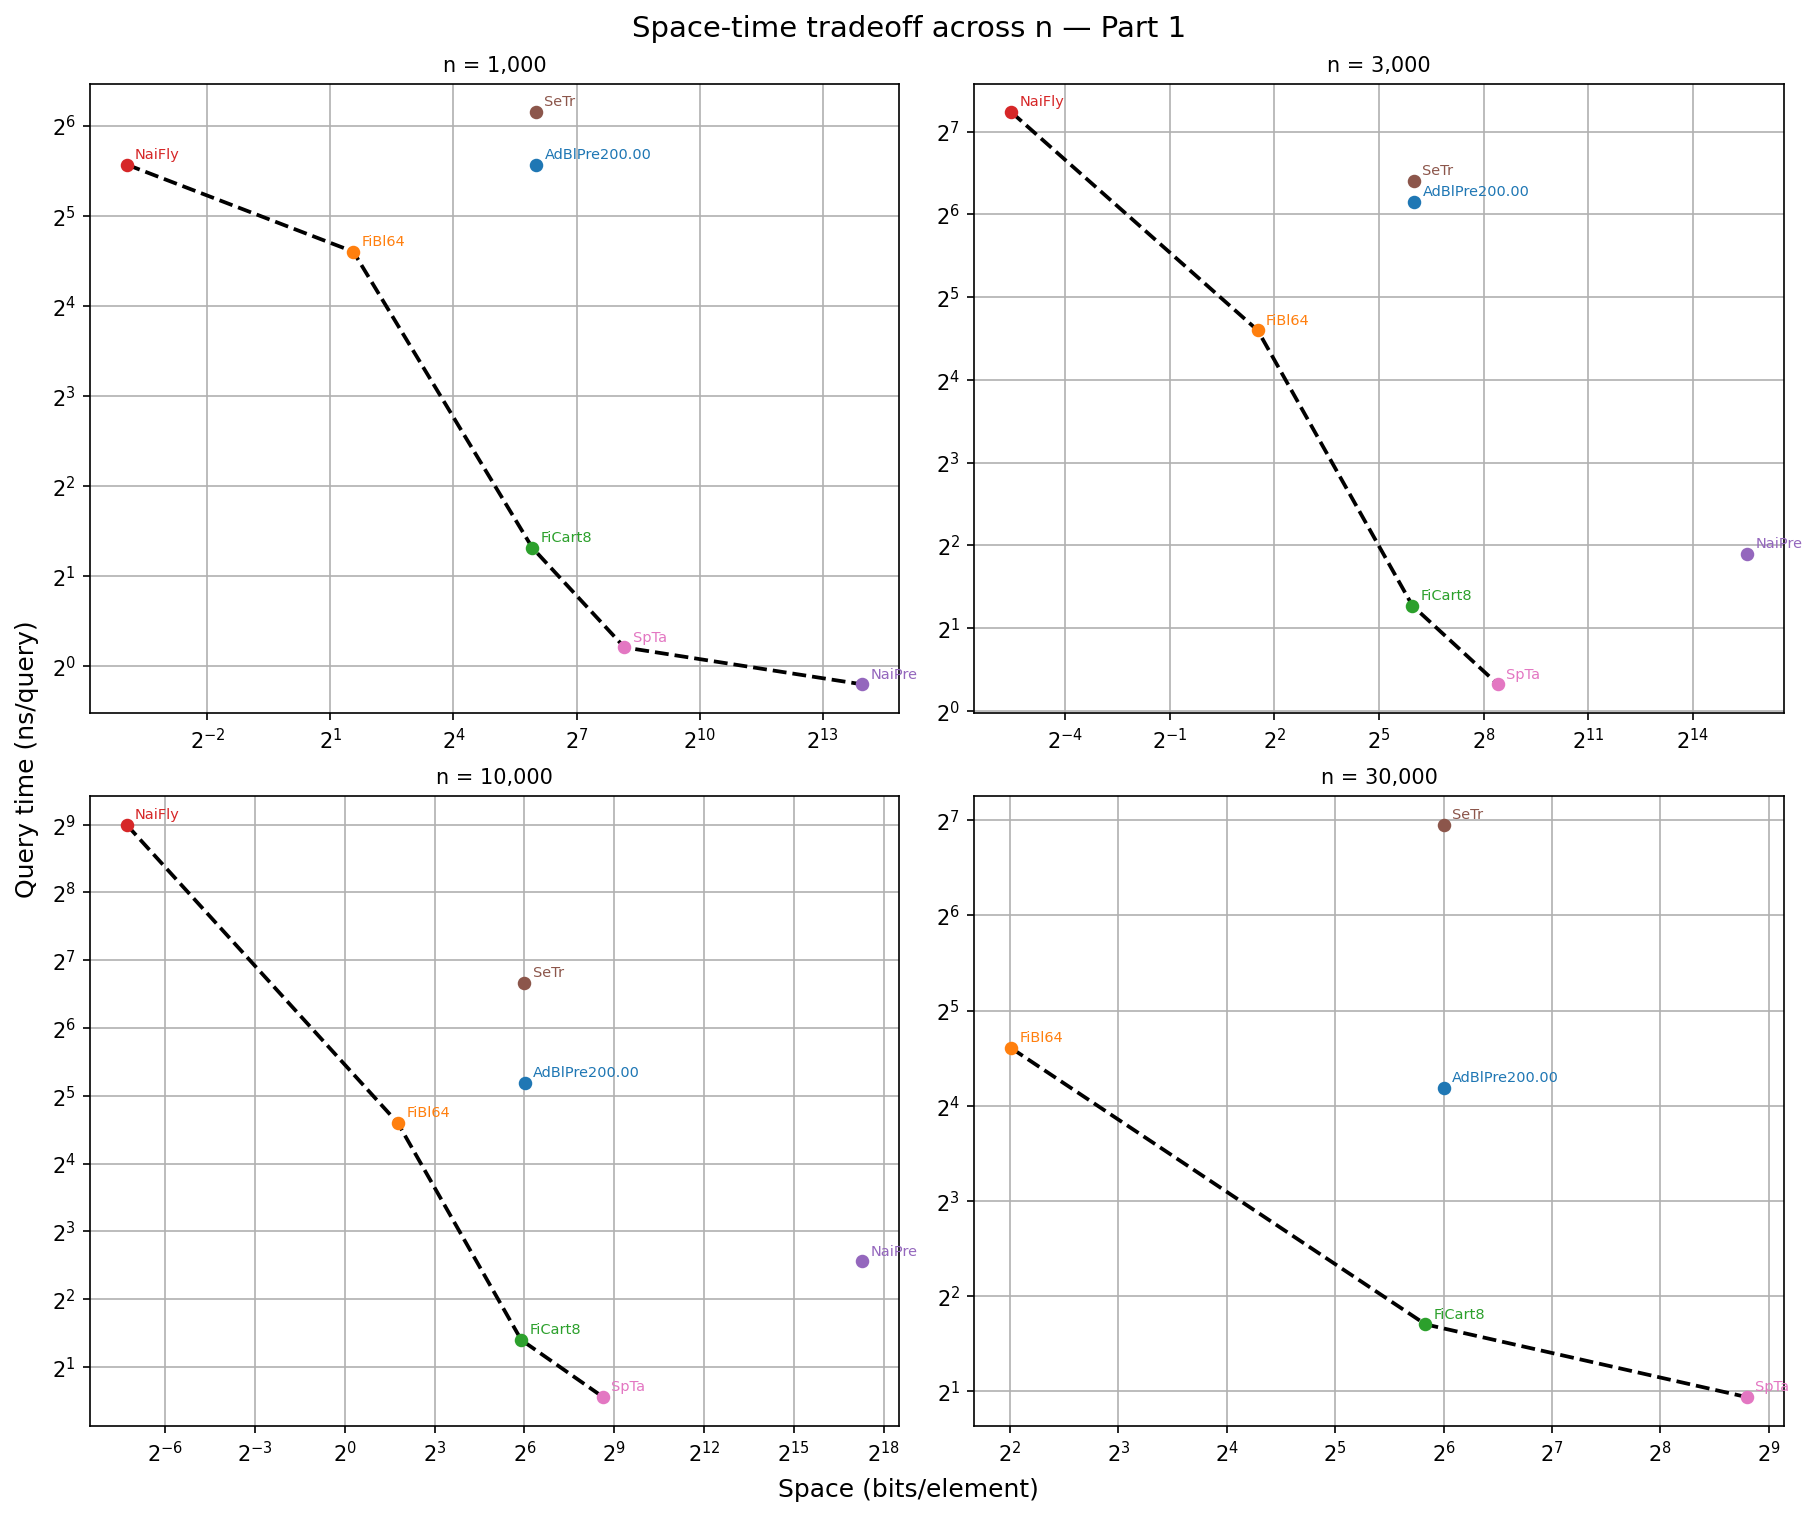
\includegraphics[width=\linewidth]{../plots/main/space_time_tradeoff_by_n_1.png}
	\caption{space-time trade-off for n's between 1000 and 30,000}
	\label{fig:tradeoff81}
	\centering
	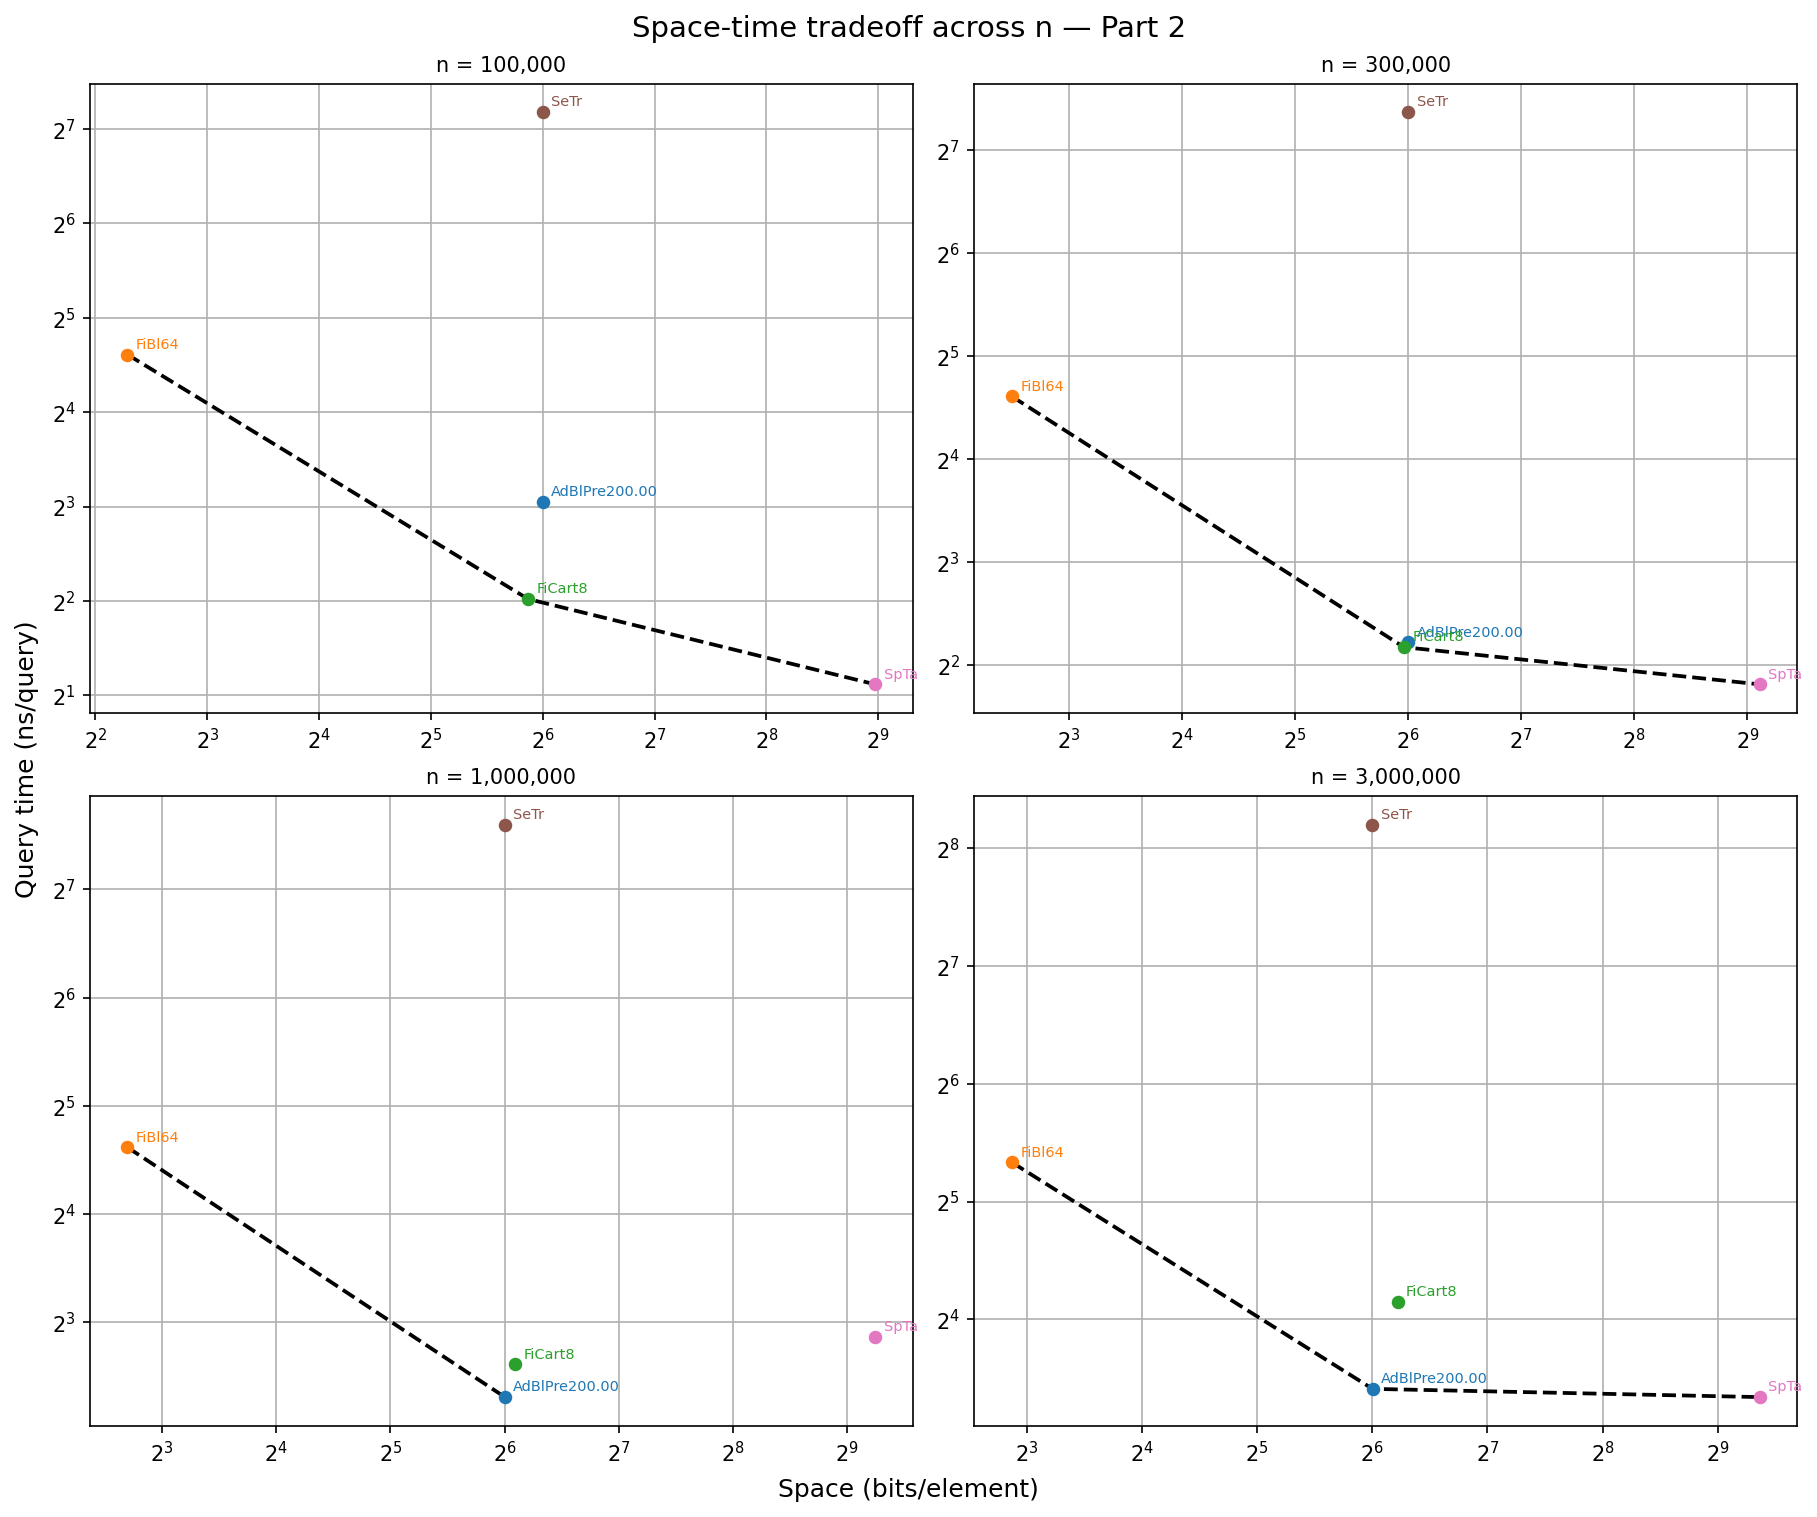
\includegraphics[width=\linewidth]{../plots/main/space_time_tradeoff_by_n_2.png}
	\caption{space-time trade-off for n's between 100,000 and 3,000,000}
	\label{fig:tradeoff82}
\end{figure}


\clearpage

\appendix

\section{Non-Precompute Block-Size Selection}
\label{app:block-selection-nonprecompute}

\begin{figure}[H]
	\centering
	\captionsetup{skip=2pt}

	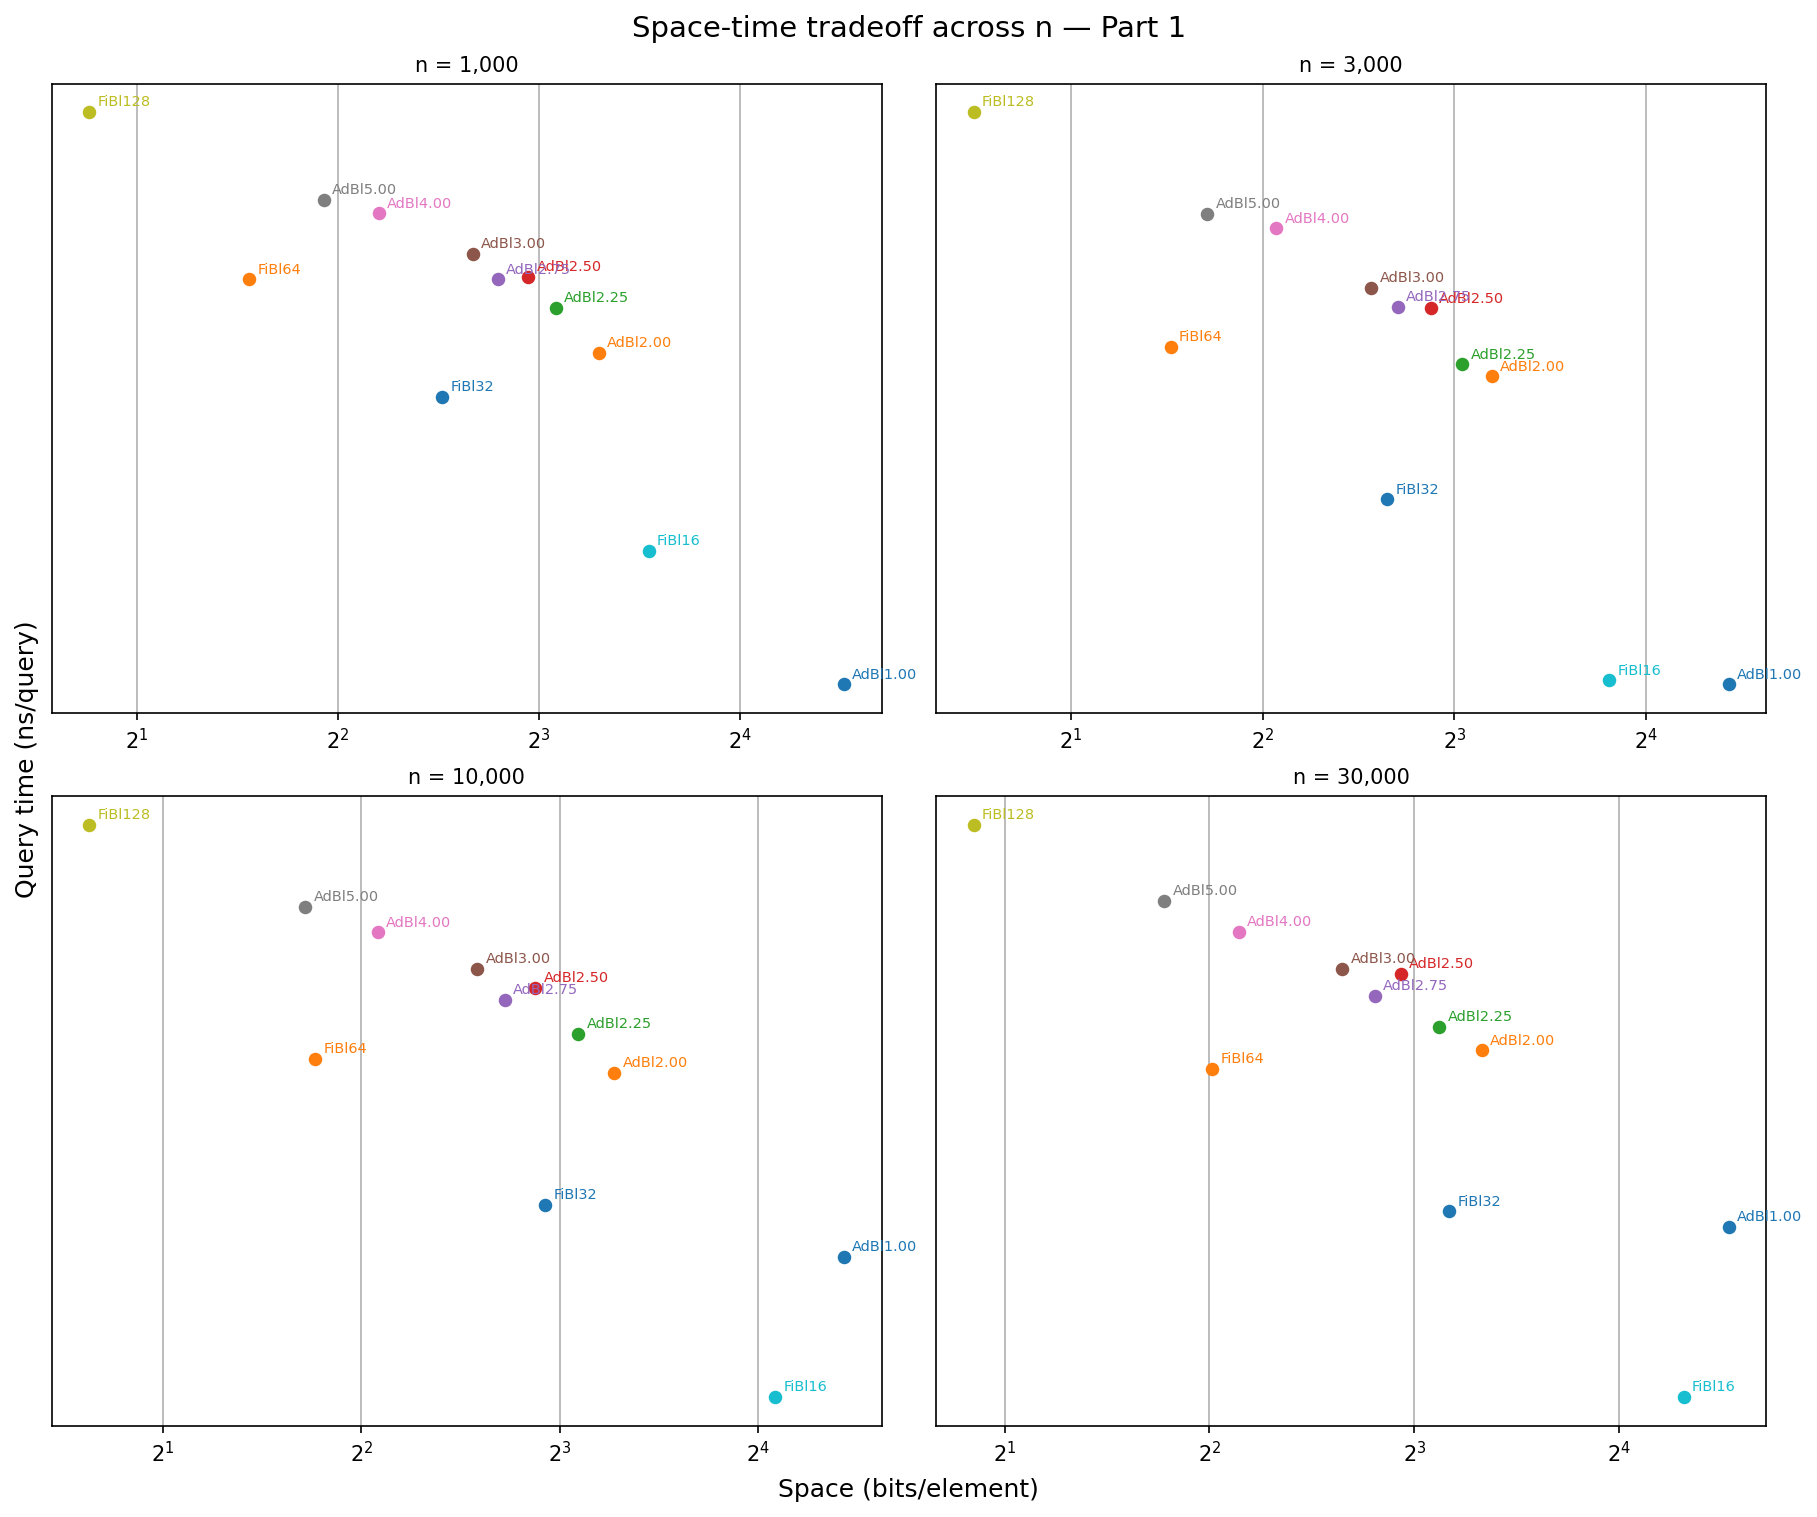
\includegraphics[width=.8\linewidth]
	{../plots/nonprecompute_blocks_fixed_adaptive/space_time_tradeoff_by_n_1.png}
	\caption{Space-time trade-off for different values of \(n\).}
	\label{fig:appendixAtradeoff1}

	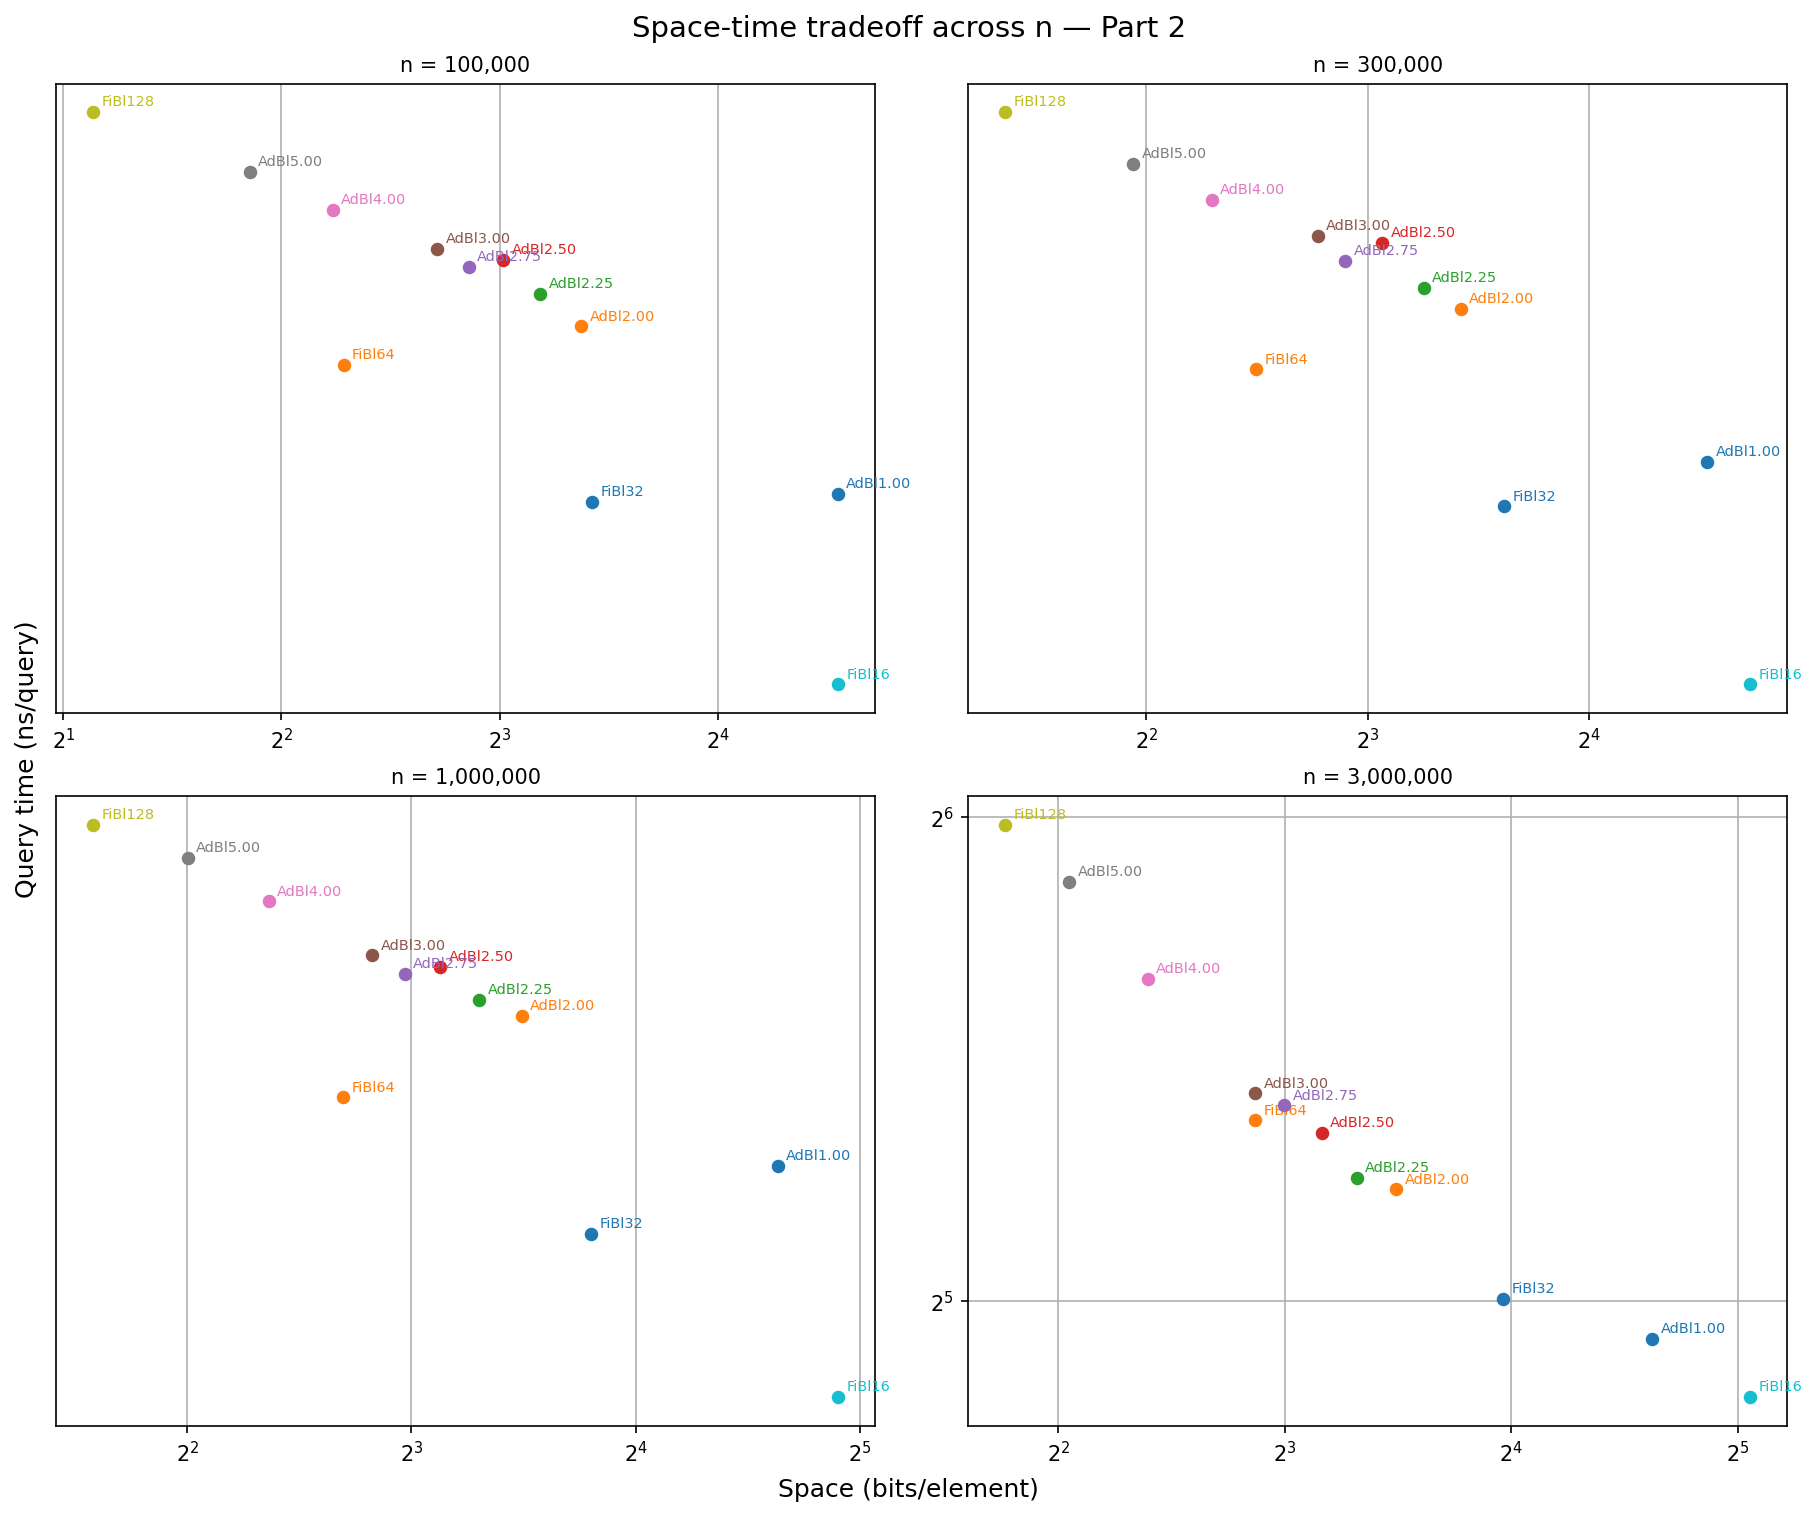
\includegraphics[width=.8\linewidth]
	{../plots/nonprecompute_blocks_fixed_adaptive/space_time_tradeoff_by_n_2.png}
	\caption{Space-time trade-off for different values of \(n\).}
	\label{fig:appendixAtradeoff2}
\end{figure}

\newpage
\section{Precompute Block-Size Selection: Overall Comparison}
\label{app:block-selection-precompute}

\begin{figure}[H]
	\centering
	\captionsetup{skip=2pt}

	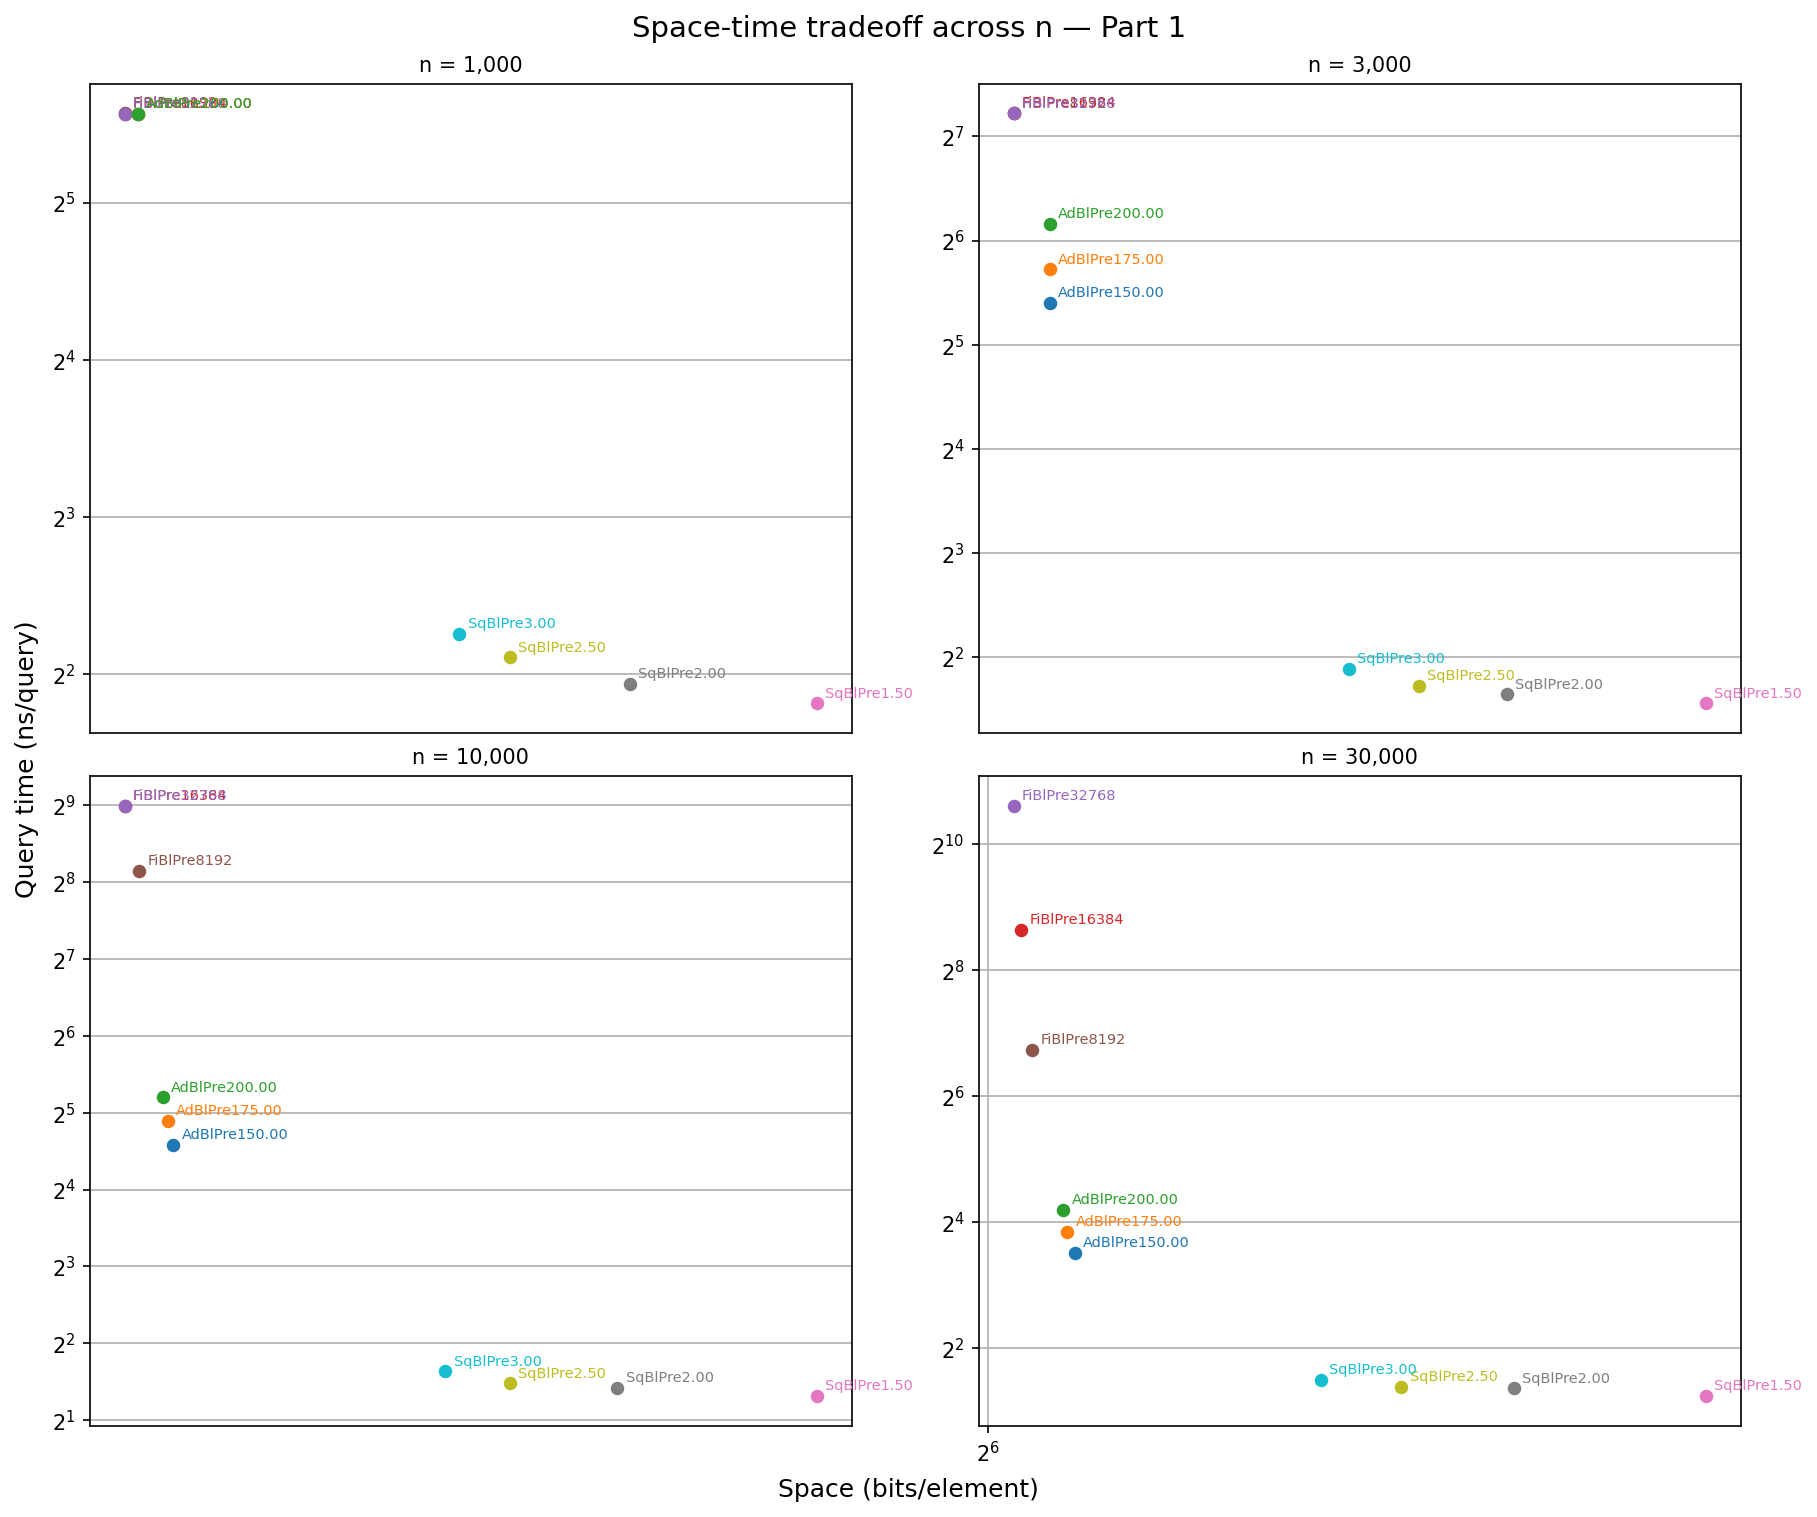
\includegraphics[width=.8\linewidth]
	{../plots/precompute_blocks_overall/space_time_tradeoff_by_n_1.png}
	\caption{Space-time trade-off for different values of \(n\).}
	\label{fig:appendixBtradeoff1}

	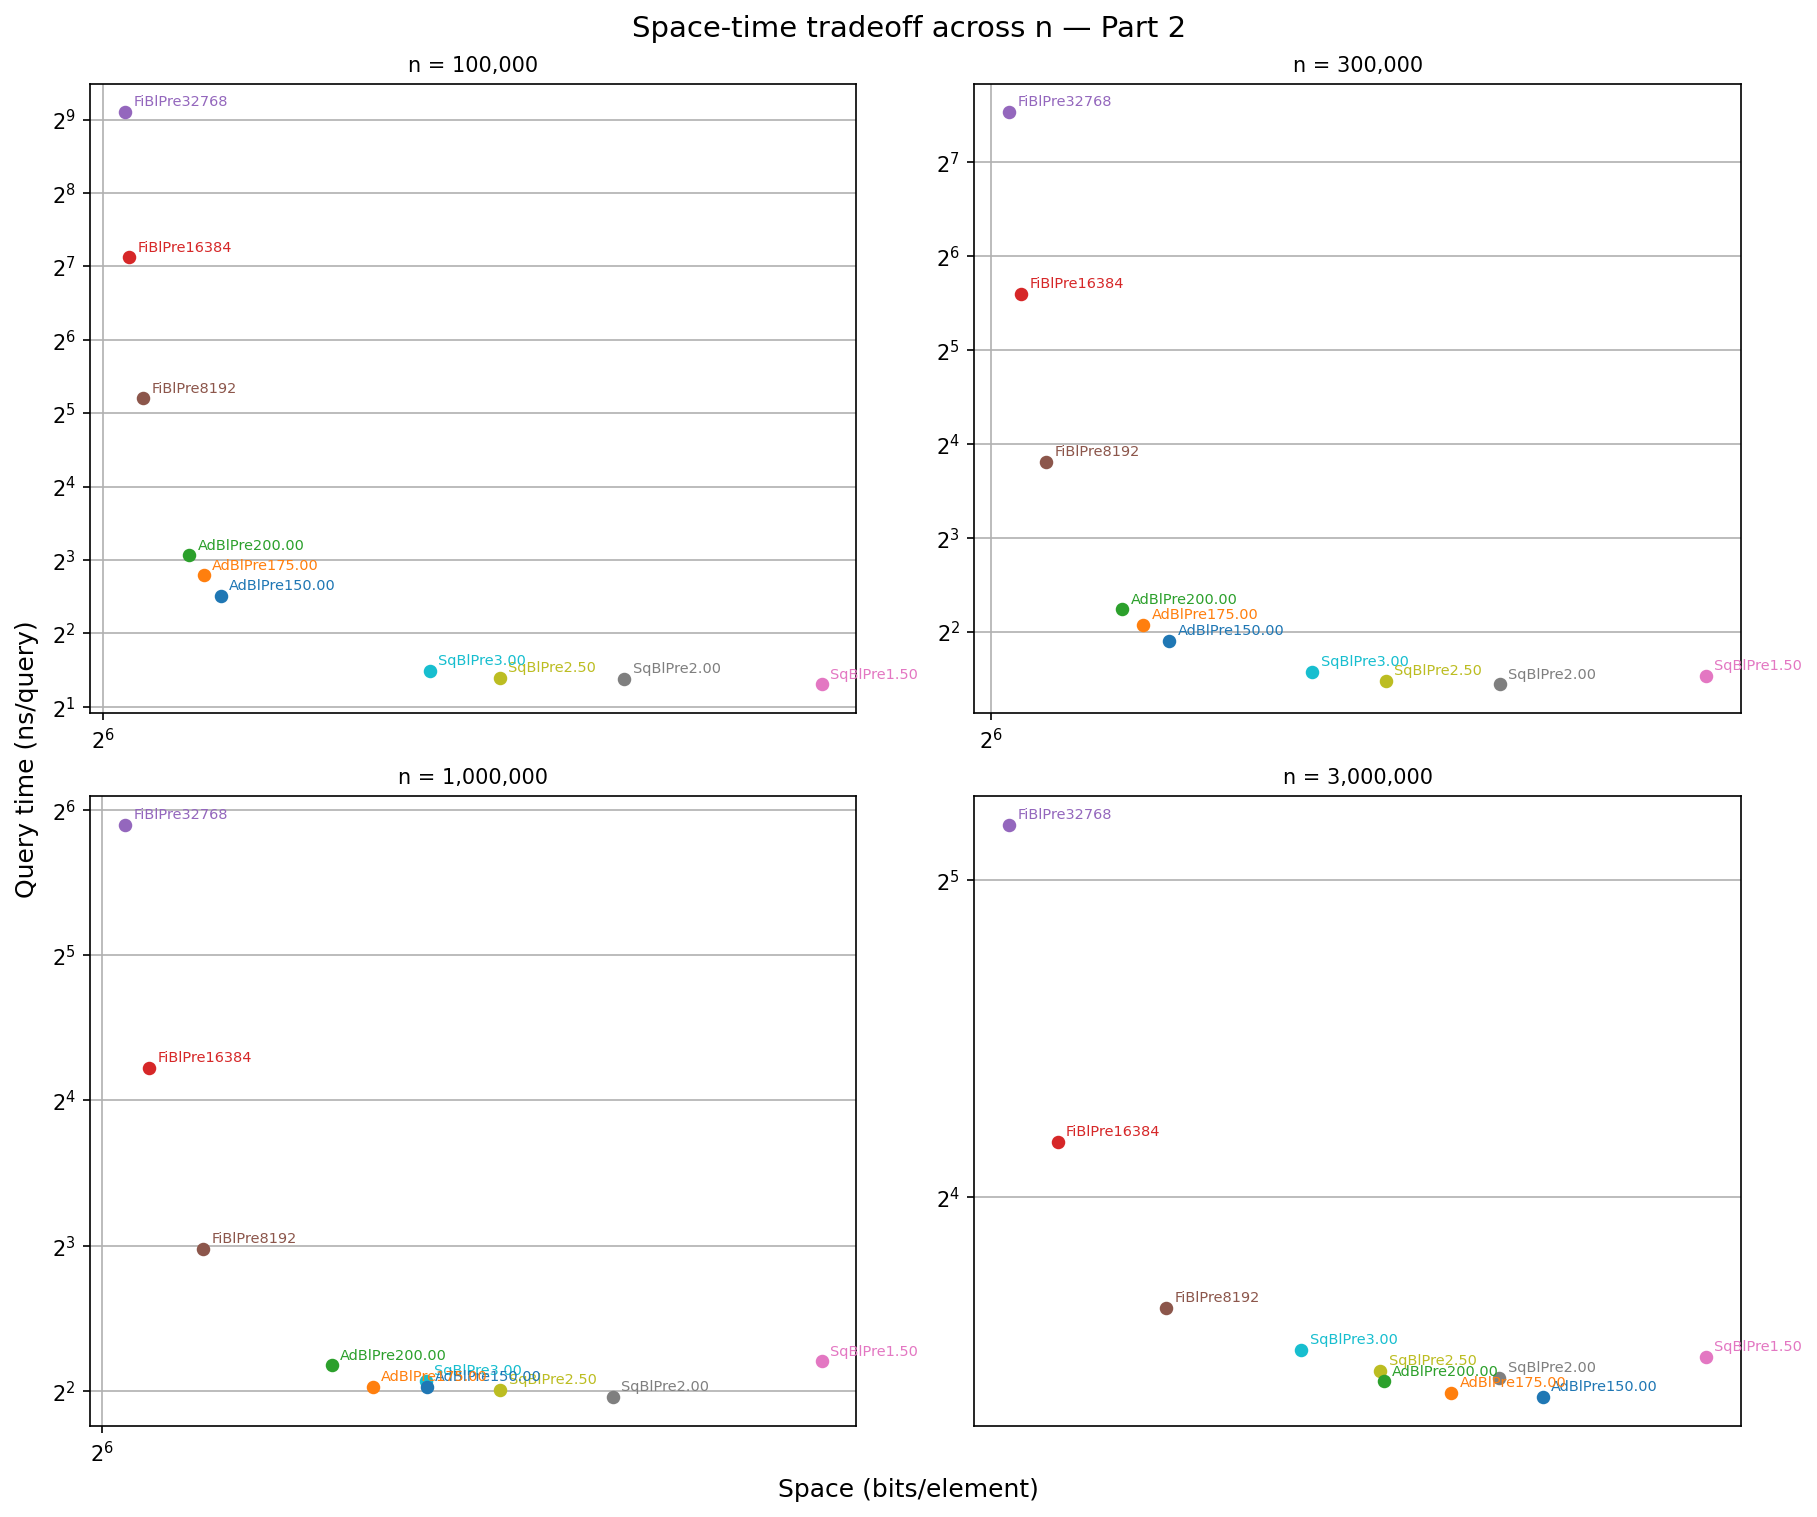
\includegraphics[width=.8\linewidth]
	{../plots/precompute_blocks_overall/space_time_tradeoff_by_n_2.png}
	\caption{Space-time trade-off for different values of \(n\).}
	\label{fig:appendixBtradeoff2}
\end{figure}

\newpage
\subsection{Fixed-Size Comparison}
\label{app:block-selection-precompute-fixed}

\begin{figure}[H]
	\centering
	\captionsetup{skip=2pt}

	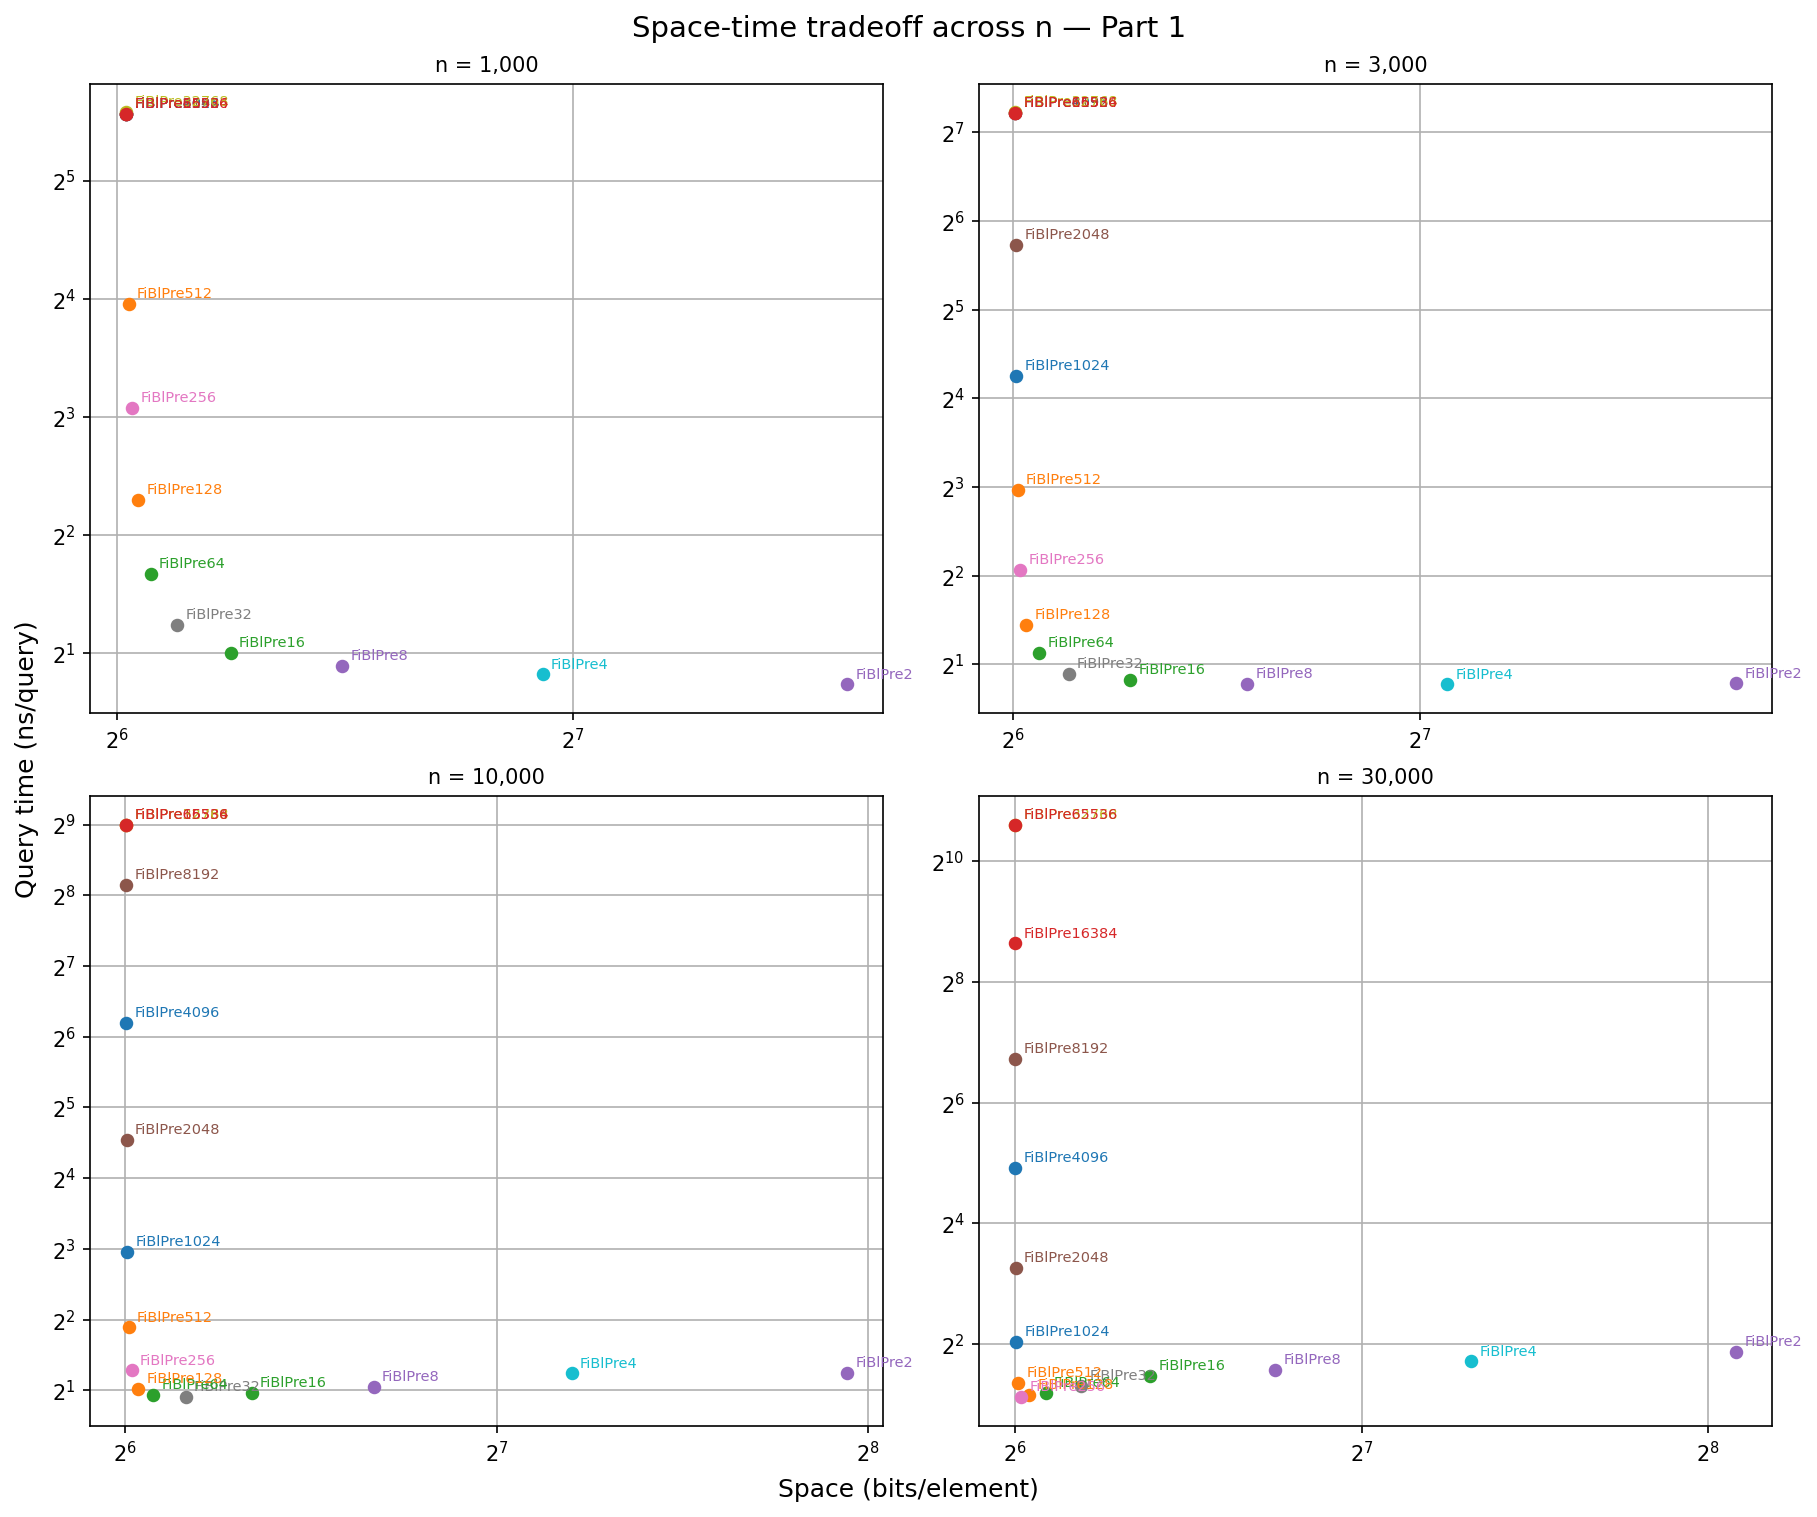
\includegraphics[width=.8\linewidth]
	{../plots/precompute_blocks_fixed/space_time_tradeoff_by_n_1.png}
	\caption{Space-time trade-off for different values of \(n\).}
	\label{fig:appendixB1tradeoff1}

	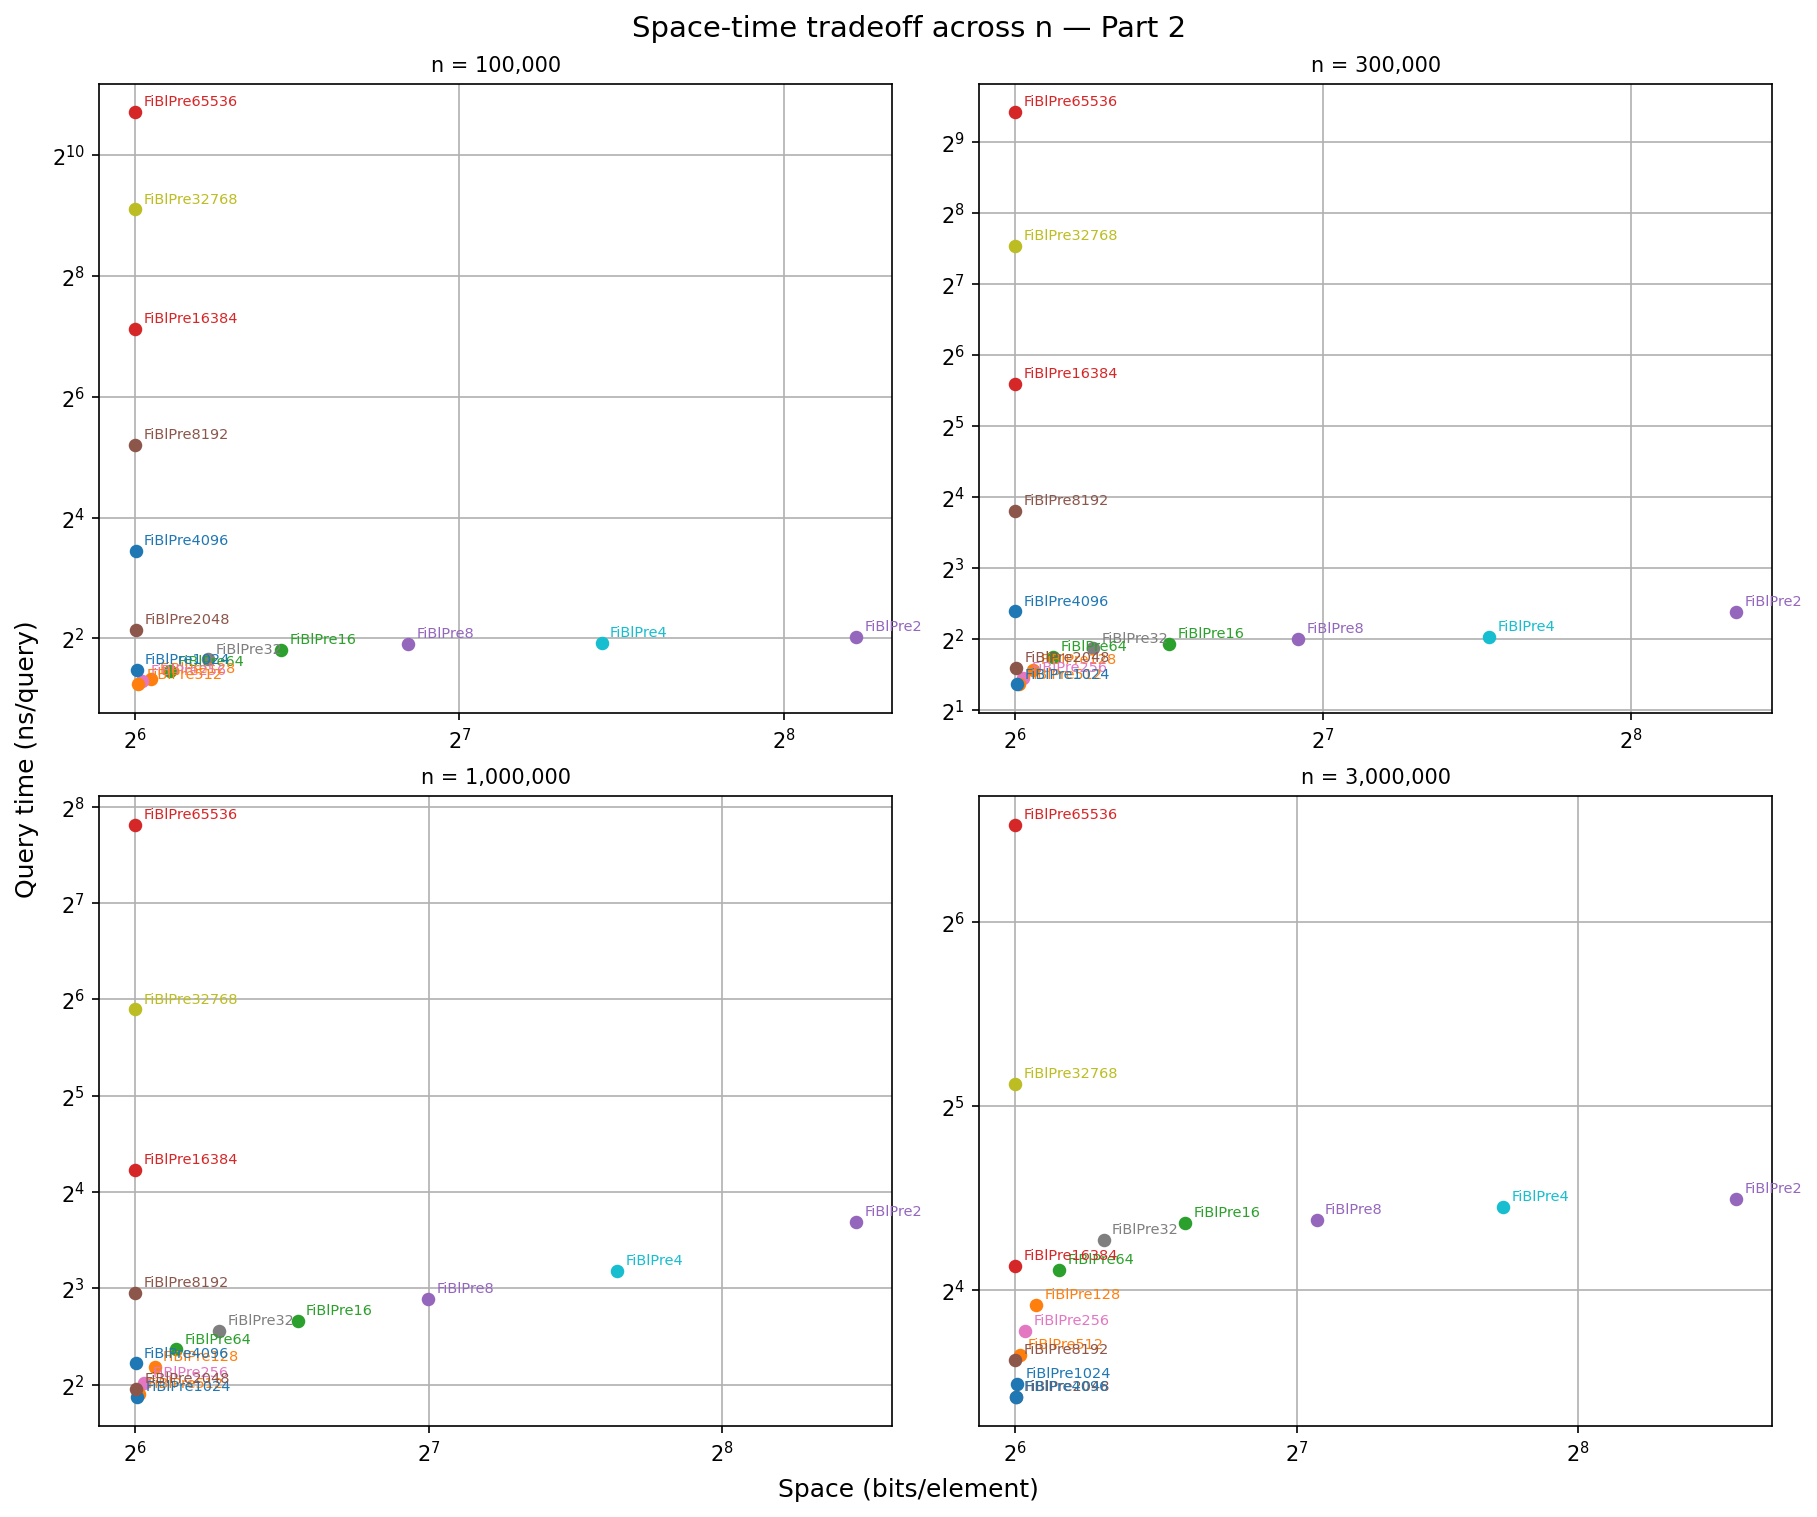
\includegraphics[width=.8\linewidth]
	{../plots/precompute_blocks_fixed/space_time_tradeoff_by_n_2.png}
	\caption{Space-time trade-off for different values of \(n\).}
	\label{fig:appendixB1tradeoff2}
\end{figure}

\newpage
\subsection{Adaptive Comparison}
\label{app:block-selection-precompute-adaptive}

\begin{figure}[H]
	\centering
	\captionsetup{skip=2pt}

	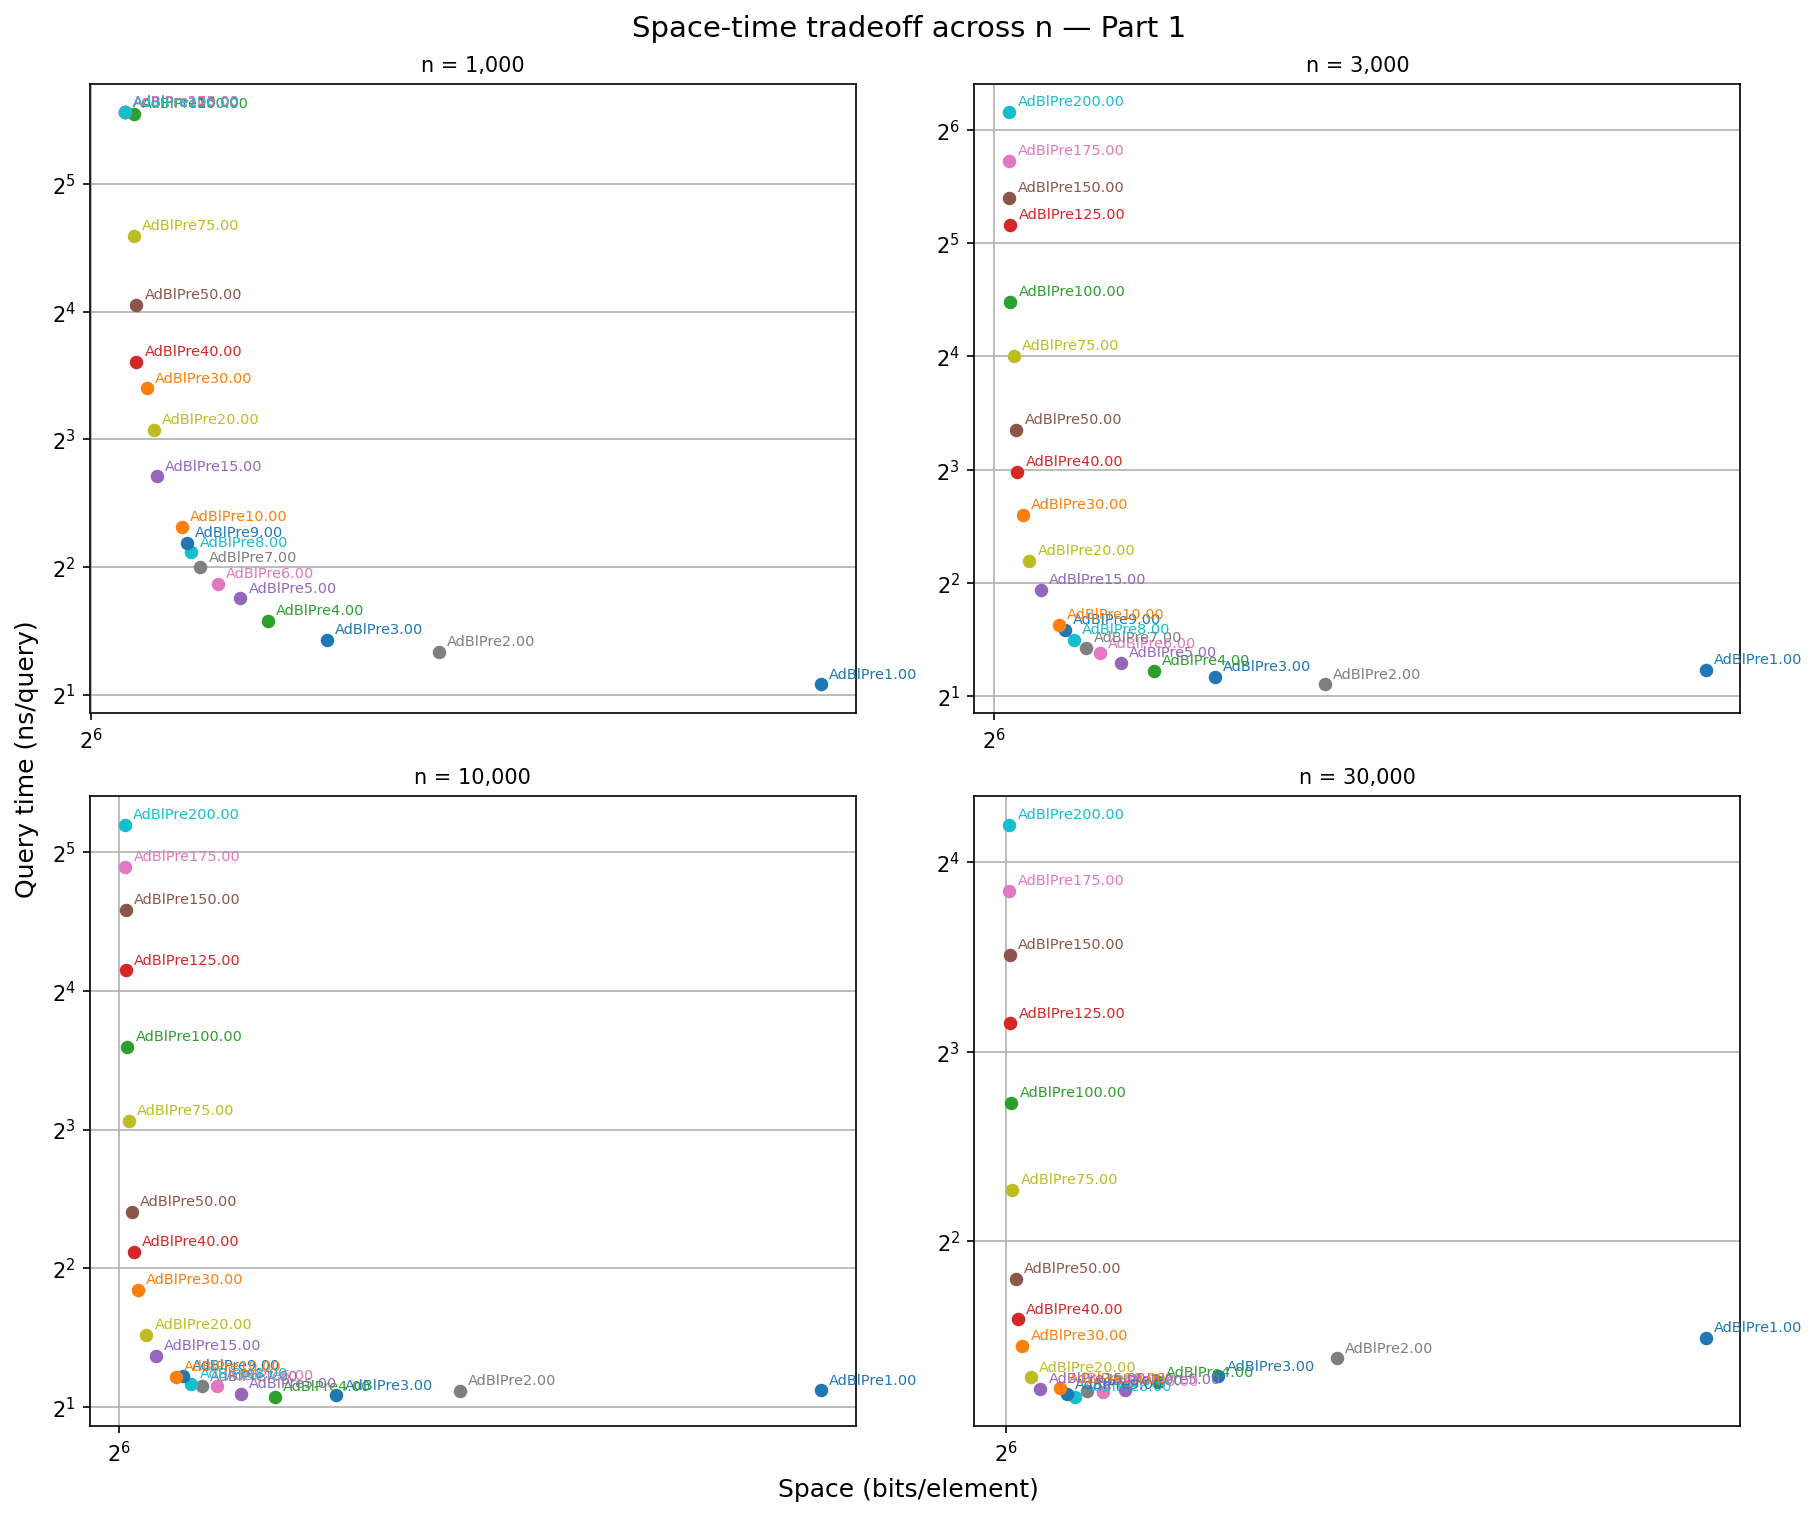
\includegraphics[width=.8\linewidth]
	{../plots/precompute_blocks_adaptive/space_time_tradeoff_by_n_1.png}
	\caption{Space-time trade-off for different values of \(n\).}
	\label{fig:appendixB2tradeoff1}

	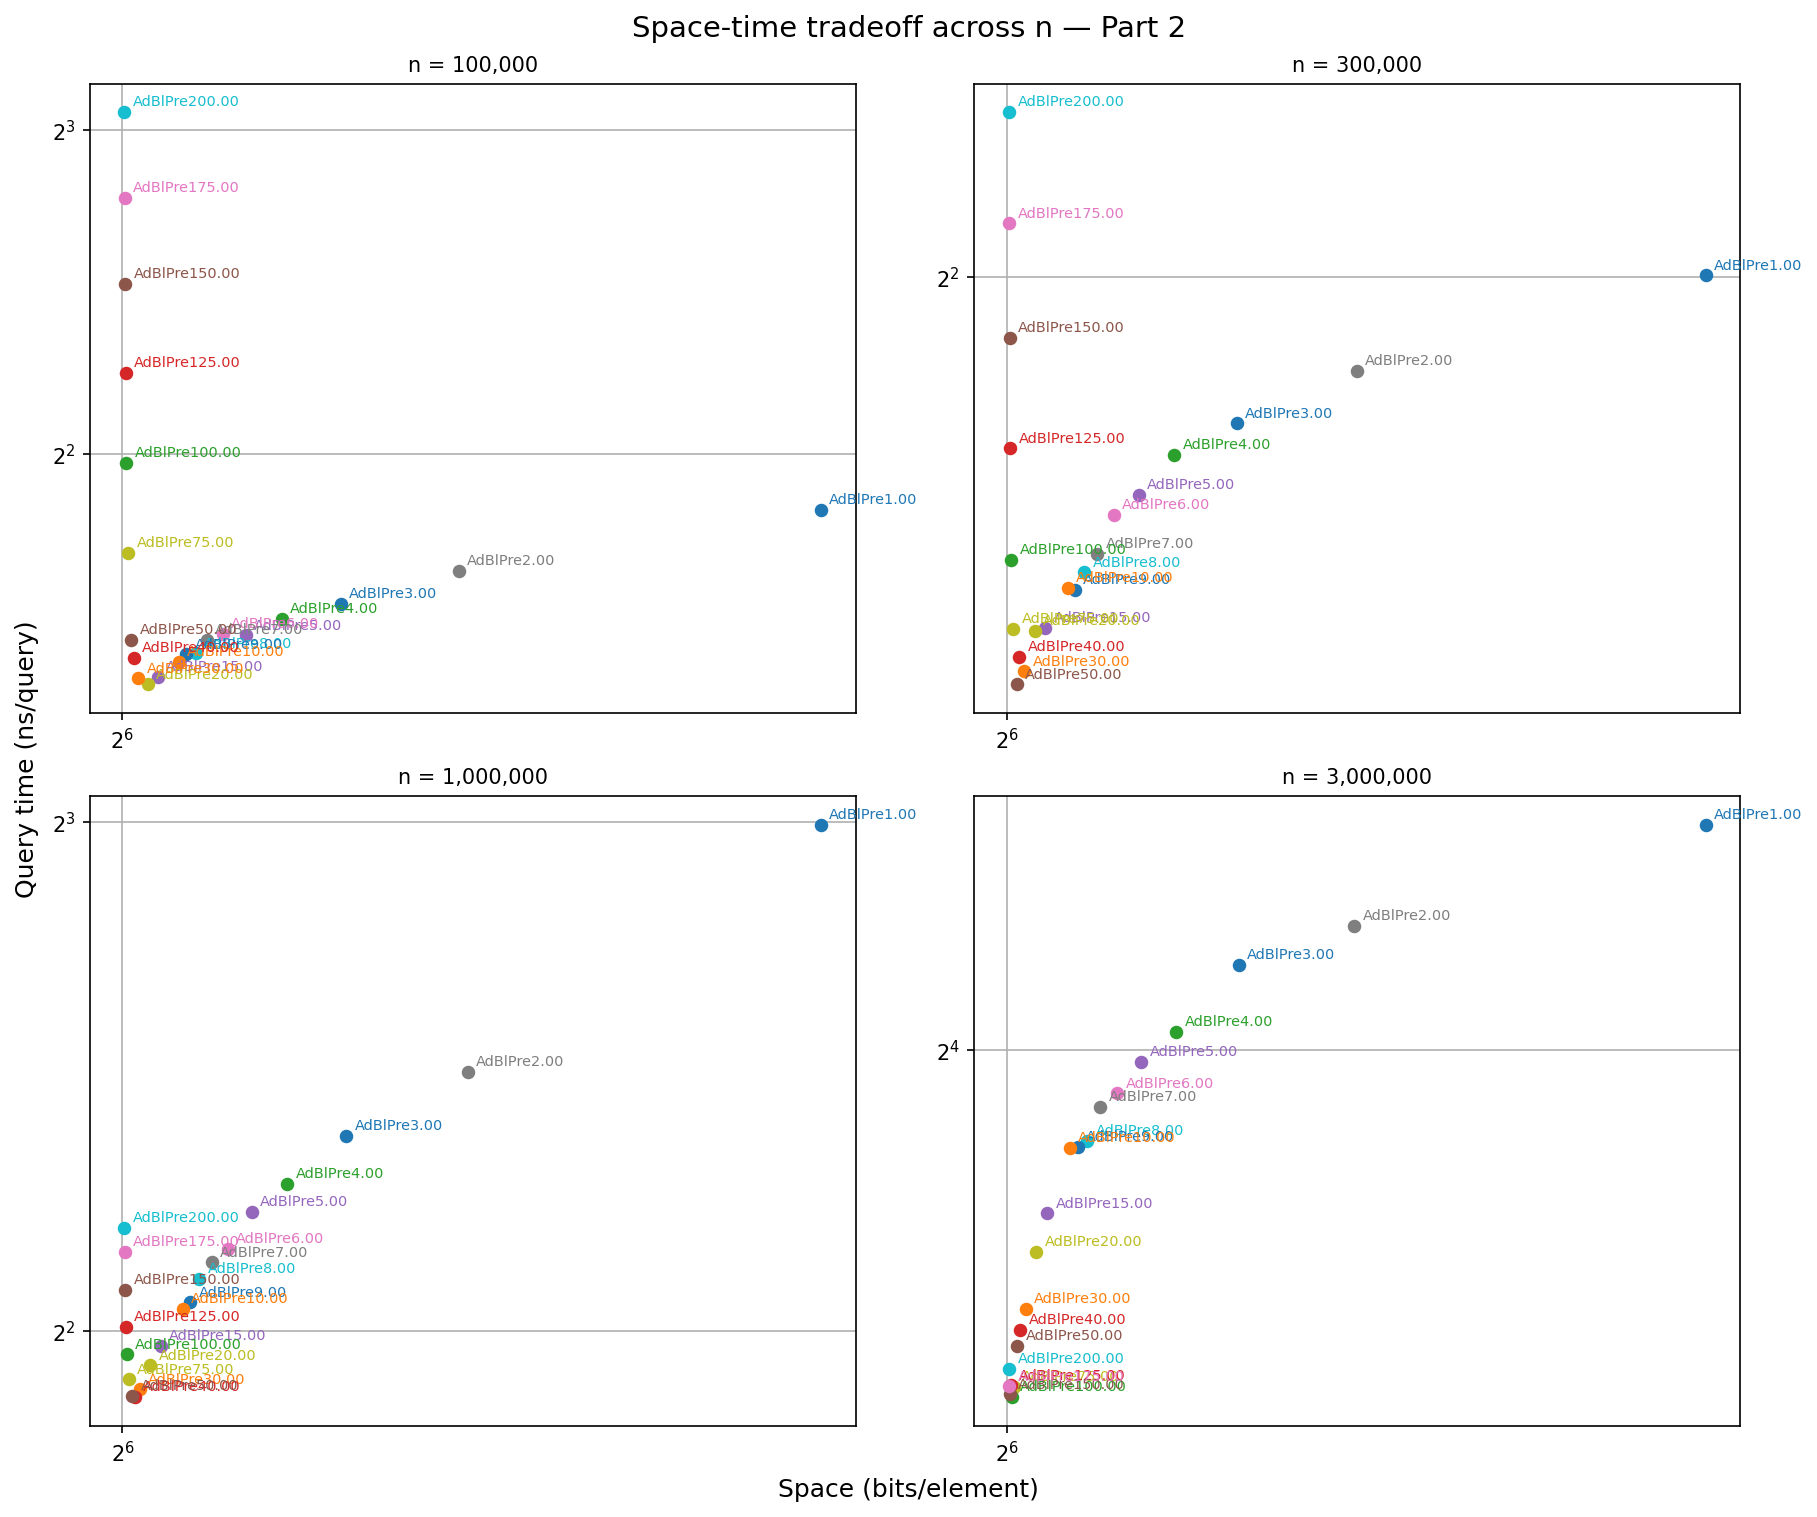
\includegraphics[width=.8\linewidth]
	{../plots/precompute_blocks_adaptive/space_time_tradeoff_by_n_2.png}
	\caption{Space-time trade-off for different values of \(n\).}
	\label{fig:appendixB2tradeoff2}
\end{figure}

\newpage
\subsection{Square-Root Comparison}
\label{app:block-selection-precompute-sqrt}

\begin{figure}[H]
	\centering
	\captionsetup{skip=2pt}

	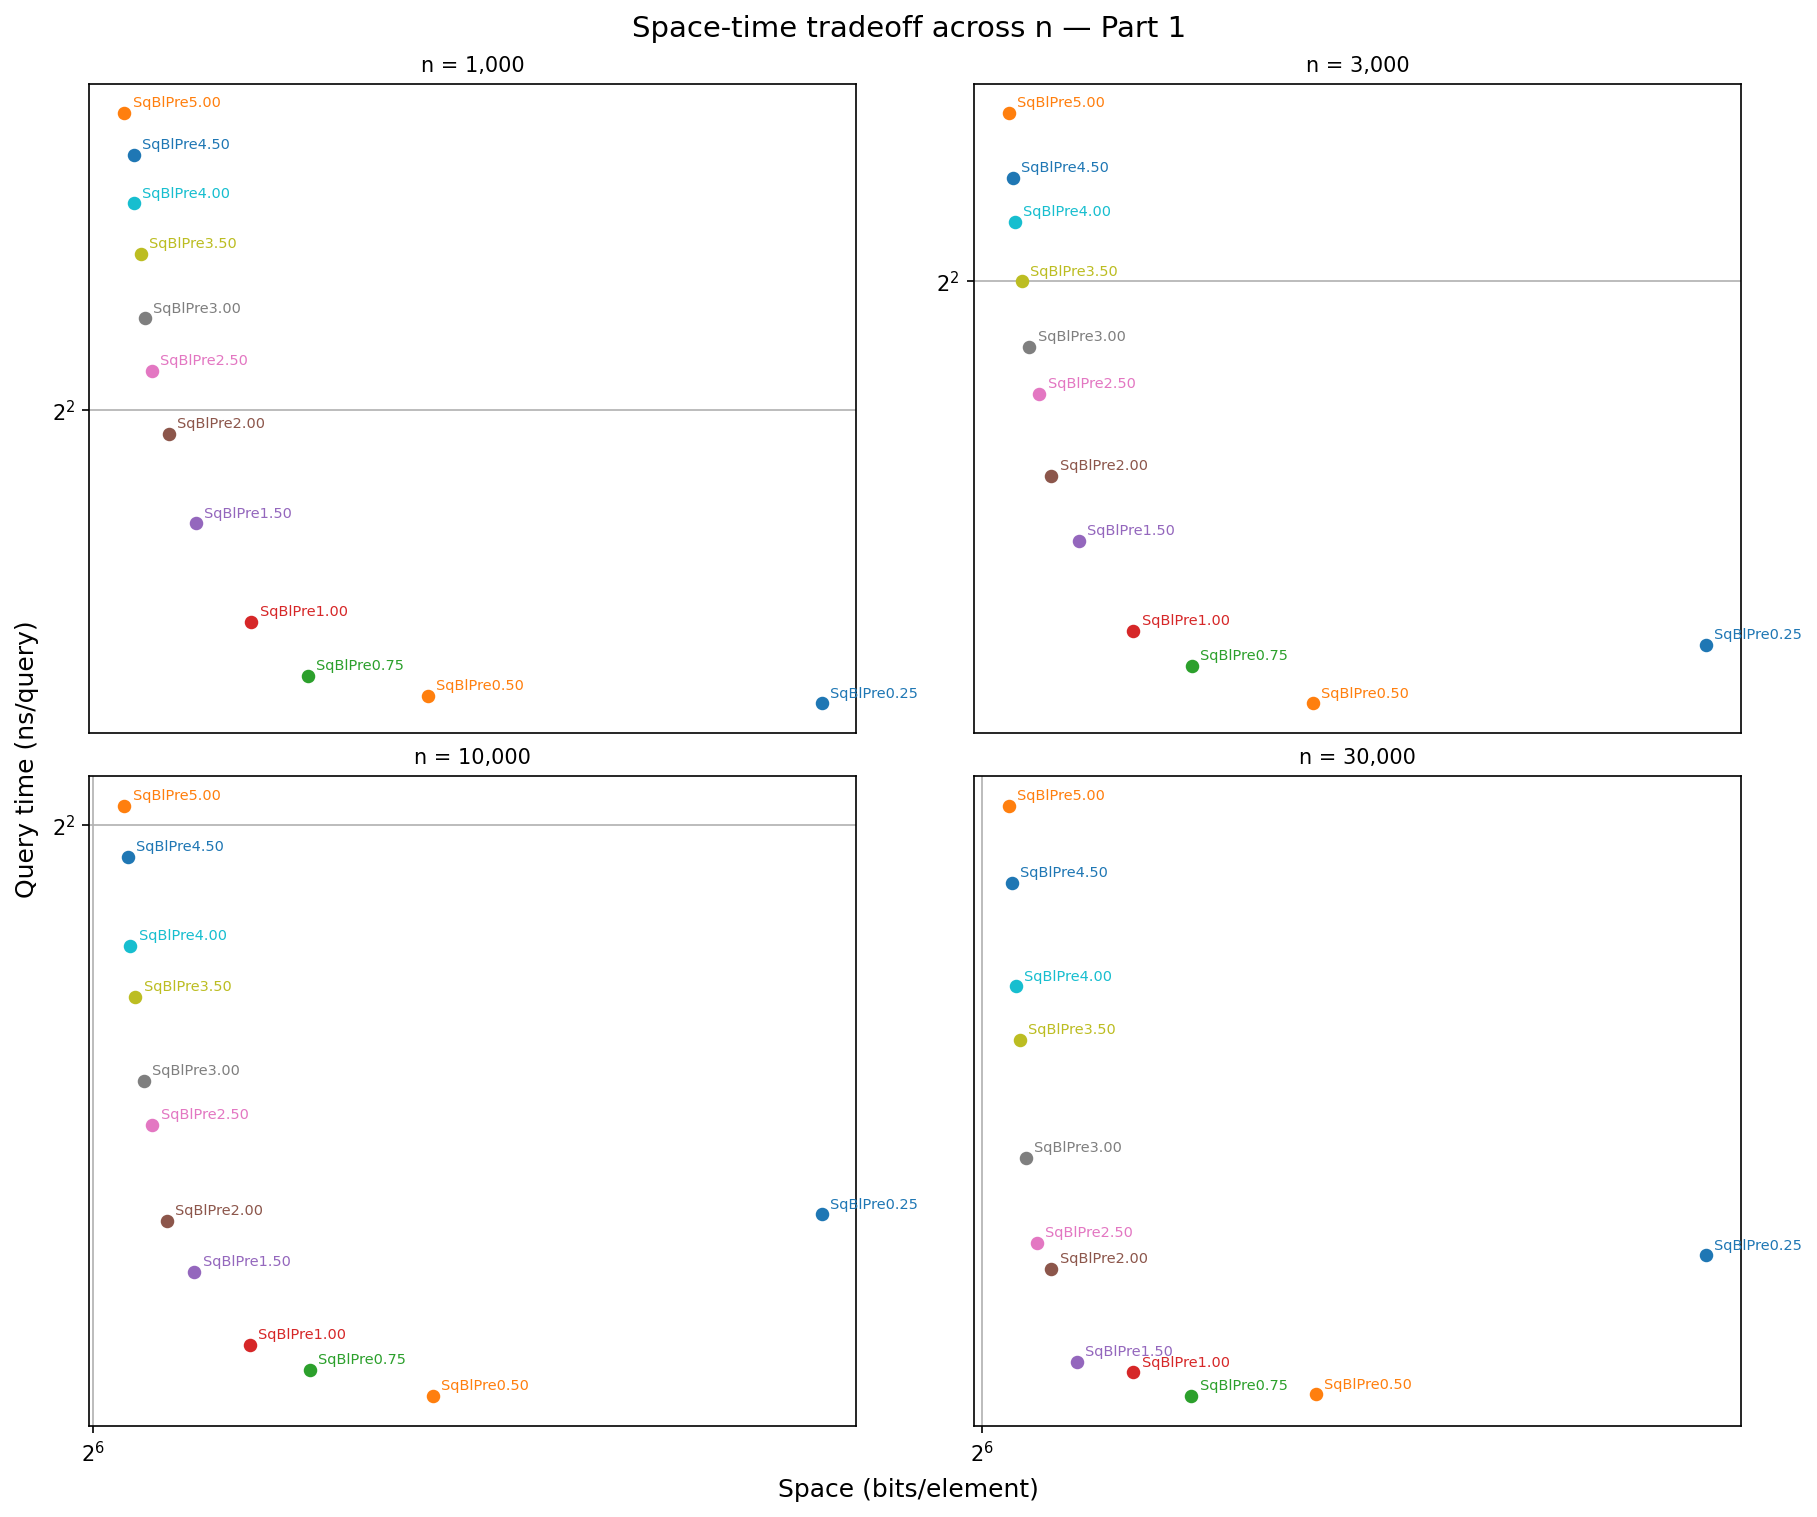
\includegraphics[width=.8\linewidth]
	{../plots/precompute_blocks_sqrt/space_time_tradeoff_by_n_1.png}
	\caption{Space-time trade-off for different values of \(n\).}
	\label{fig:appendixB3tradeoff1}

	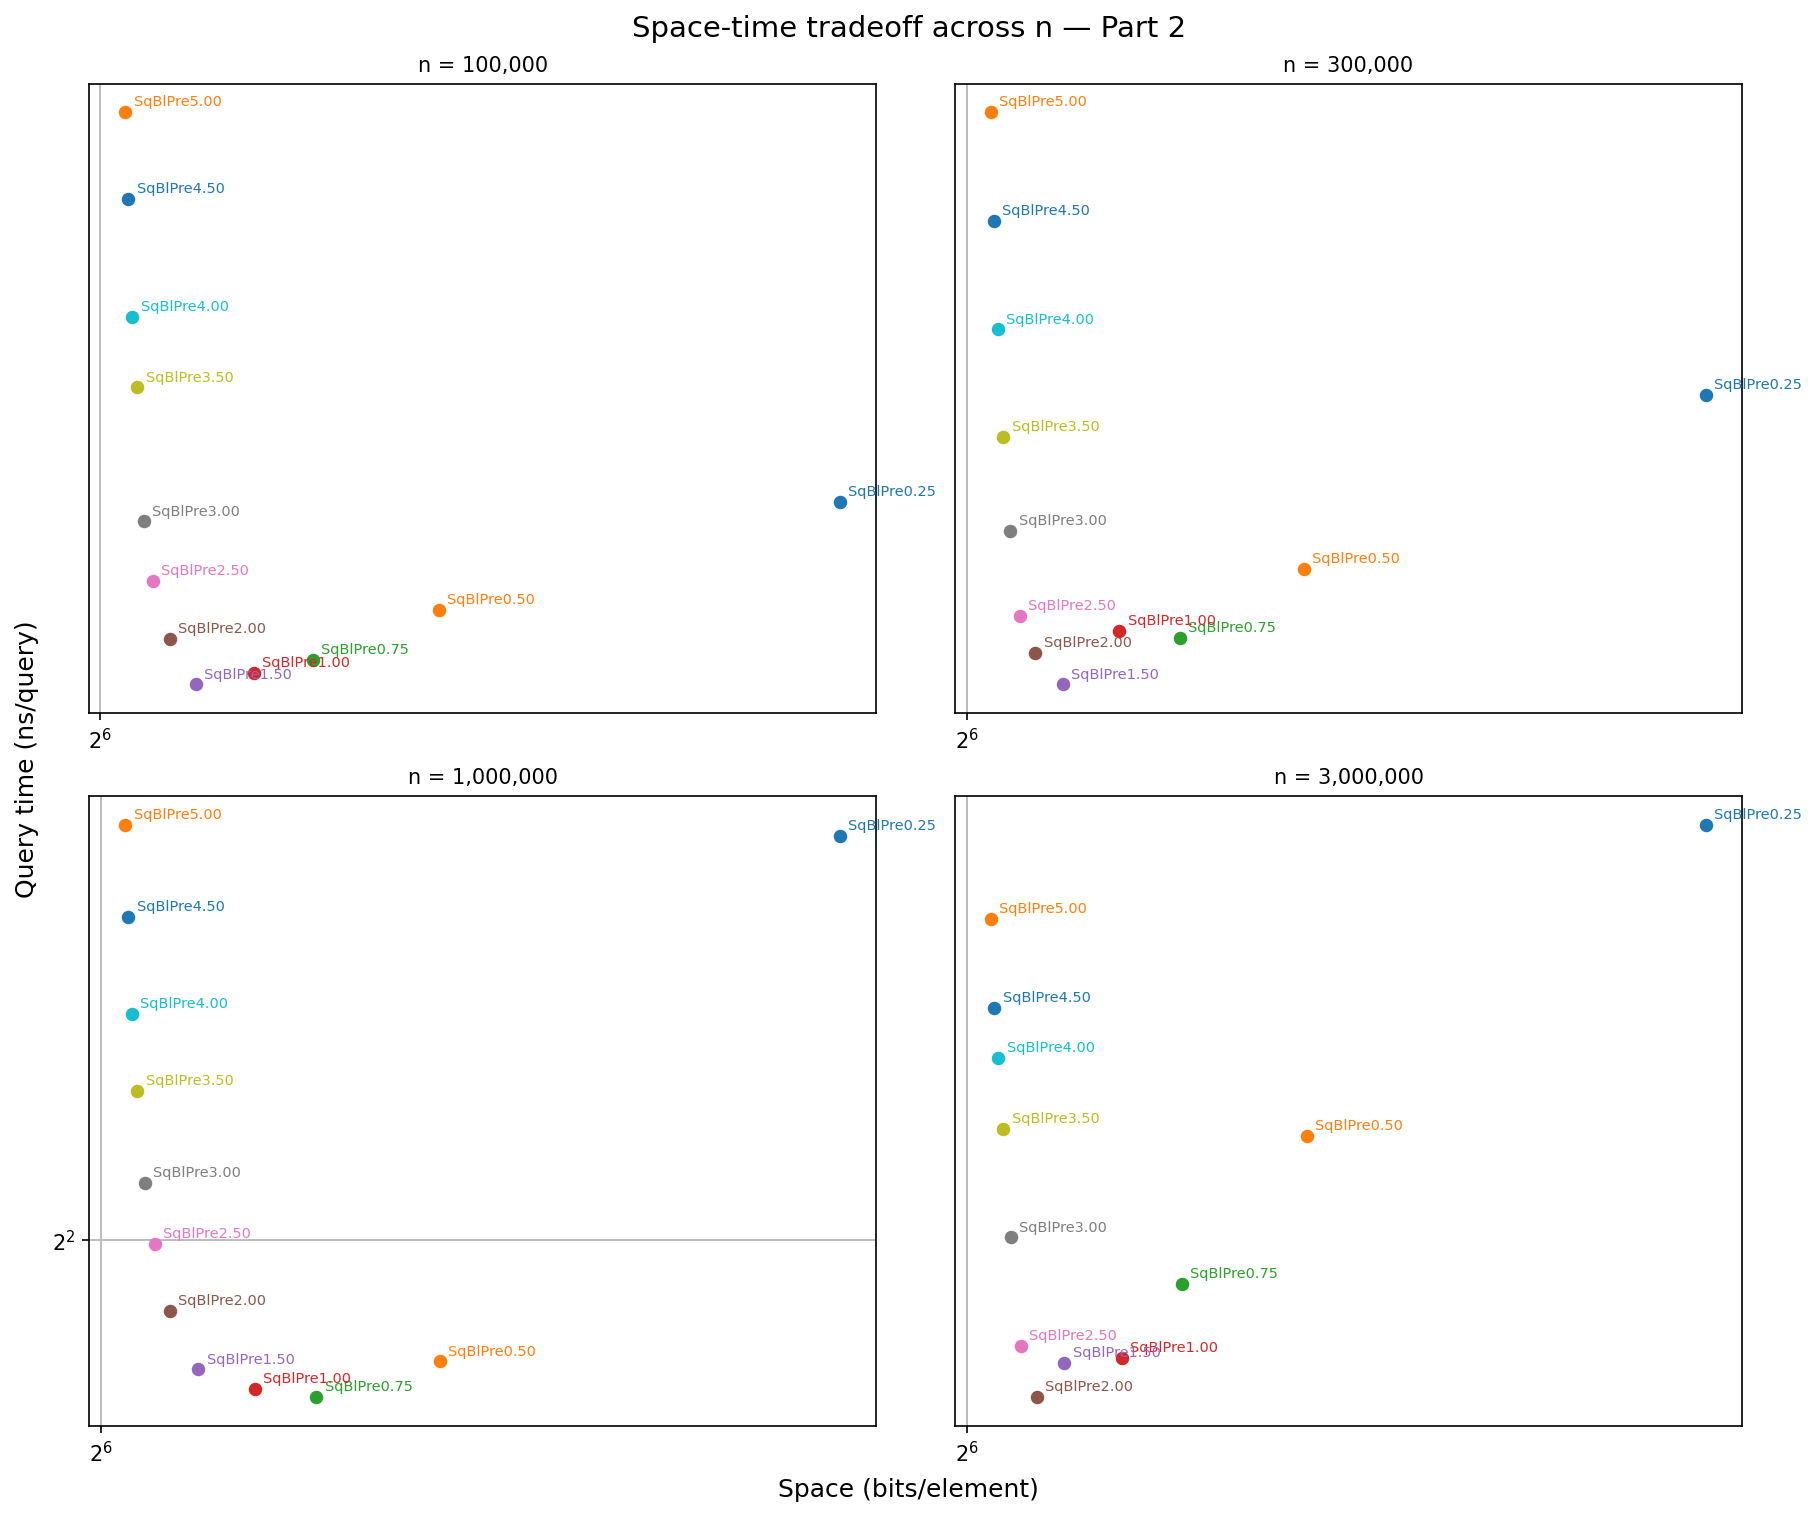
\includegraphics[width=.8\linewidth]
	{../plots/precompute_blocks_sqrt/space_time_tradeoff_by_n_2.png}
	\caption{Space-time trade-off for different values of \(n\).}
	\label{fig:appendixB3tradeoff2}
\end{figure}

\section{CartesianTree Block-Size Selection}
\label{app:block-selection-cartesian}
\begin{figure}[H]
	\centering
	\captionsetup{skip=2pt}

	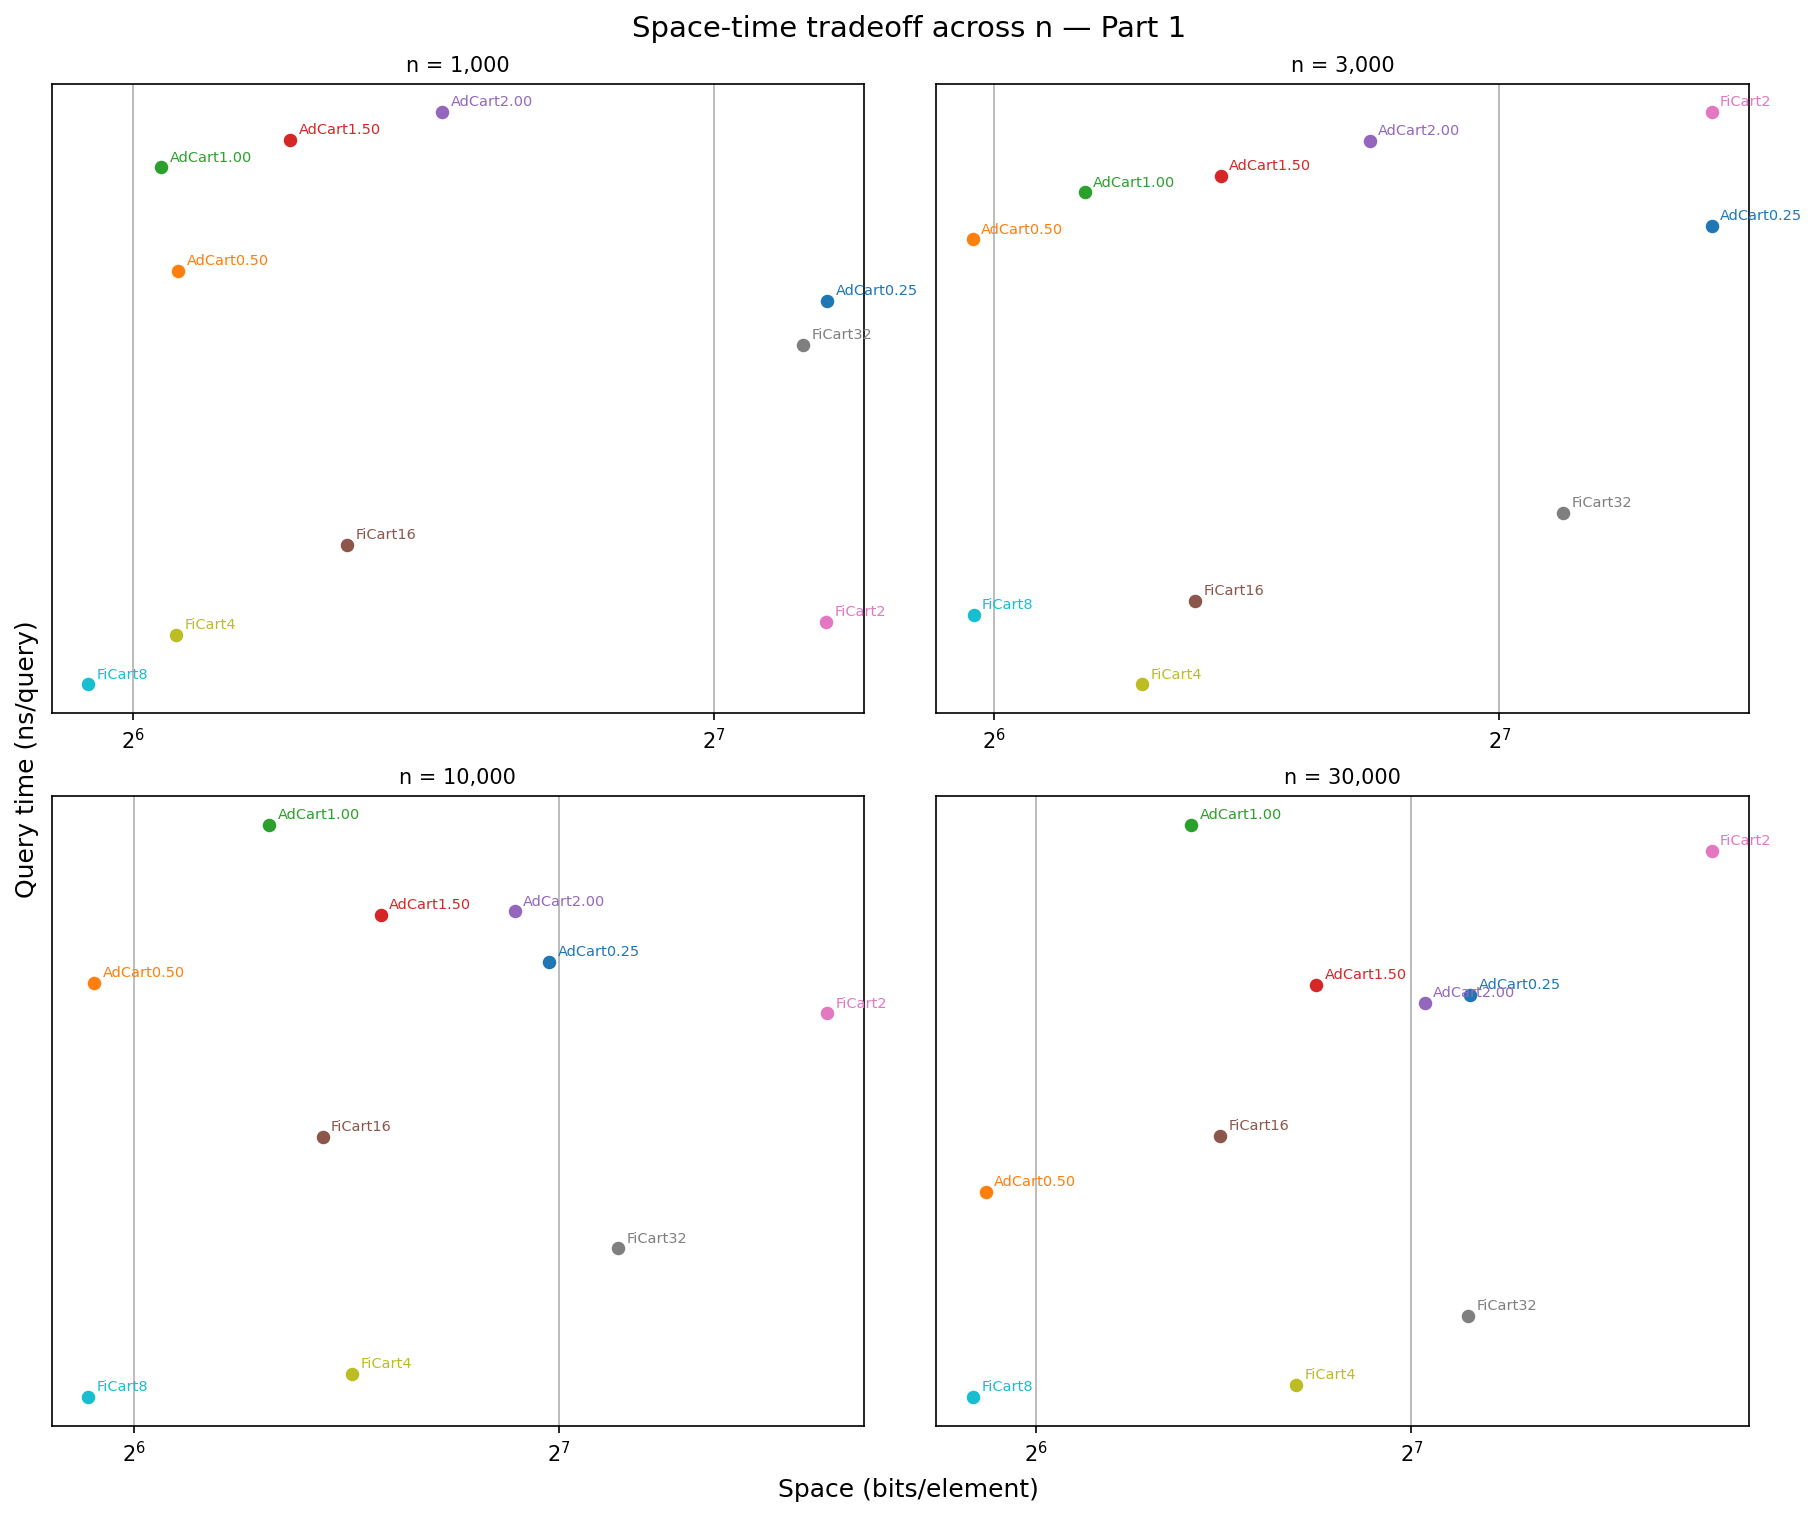
\includegraphics[width=.8\linewidth]
	{../plots/cartesian/space_time_tradeoff_by_n_1.png}
	\caption{Space-time trade-off for different values of \(n\).}
	\label{fig:appendixCtradeoff1}

	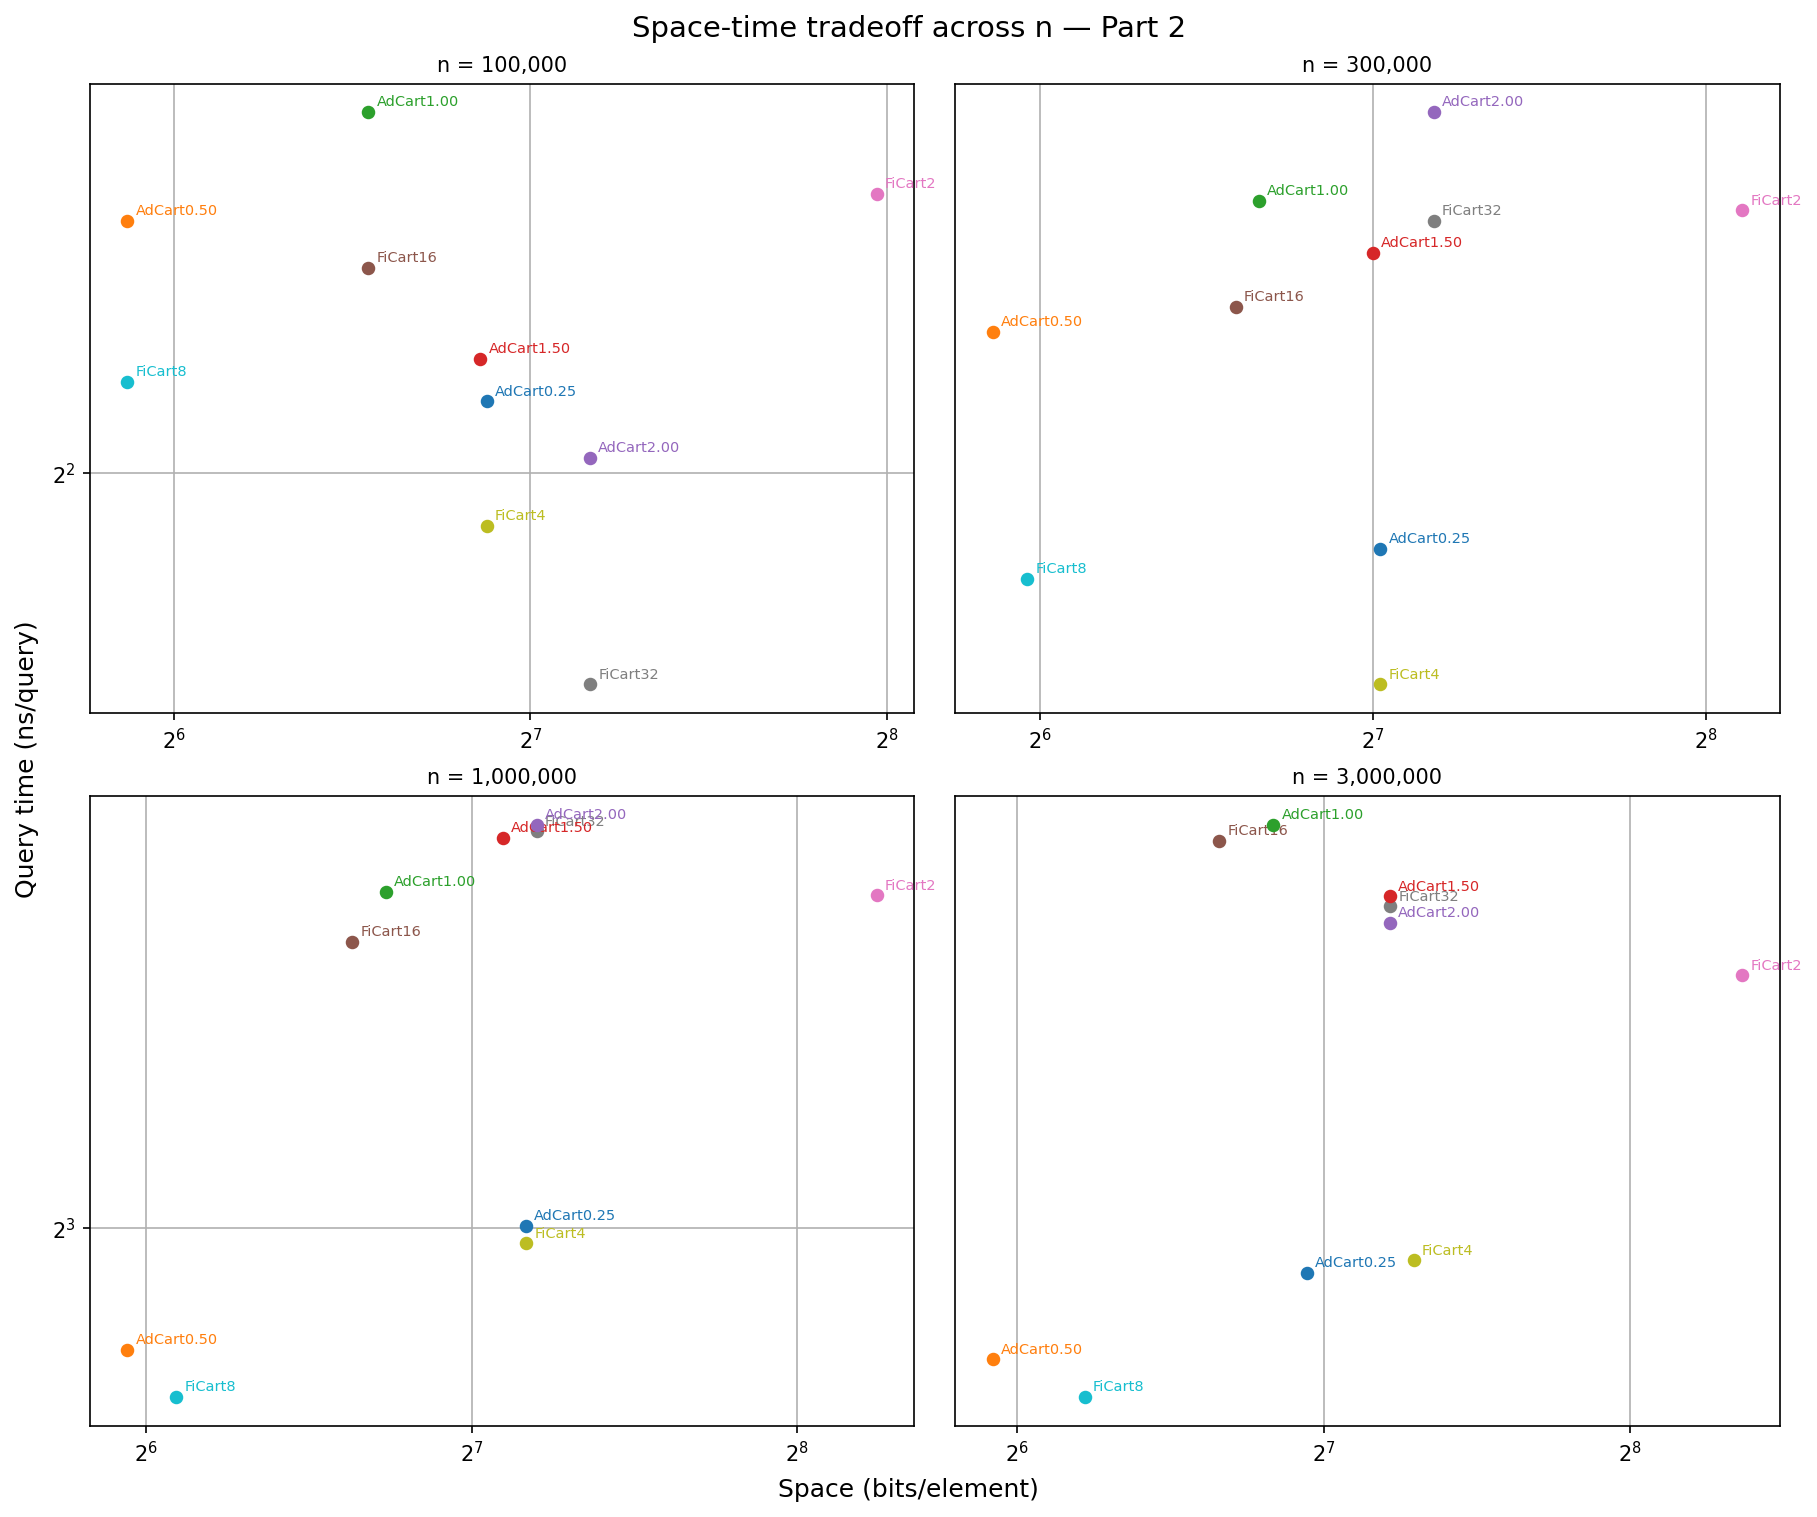
\includegraphics[width=.8\linewidth]
	{../plots/cartesian/space_time_tradeoff_by_n_2.png}
	\caption{Space-time trade-off for different values of \(n\).}
	\label{fig:appendixCtradeoff2}
\end{figure}

\end{document}




